\documentclass[11pt,article,oneside,a4paper]{memoir}
\usepackage[dutch,english]{babel}
\newcommand\Dutch[1]{`\foreignlanguage{dutch}{#1}'}
\usepackage{graphicx}

%% Determine page layout
\setlrmarginsandblock{35mm}{*}{1}
\setulmarginsandblock{35mm}{*}{1.2}
\checkandfixthelayout

%% Fonts 
%  Main text fonts: Utopia, Bera-Sans and LuxiMono
%  Remember their names, so we can use them in the text
\usepackage{fourier}
\newcommand*\rmfontname{Utopia}
\IfFileExists{berasans.sty}%
 {\usepackage[scaled=.85]{berasans}%
  \newcommand*\sffontname{Bera Sans}}%
 {\usepackage[scaled=.9]{helvet}%
  \newcommand*\sffontname{Helvetica}}
\IfFileExists{luximono.sty}%
 {\usepackage[scaled=.85]{luximono}%
  \newcommand*\ttfontname{Luxi Mono}}%
 {\renewcommand\ttdefault{lmtt}%
  \newcommand*\ttfontname{Latin Modern Typewriter}}

%% Styling pages, sections and lists
\pagestyle{plain}
\renewcommand\chaptitlefont{\Large\sffamily}
\setsecheadstyle{\large\sffamily\raggedright}
\setparaheadstyle{\normalsize\scshape}
\setbeforeparaskip{\medskipamount}
\firmlists

%% Define some typesetting commands
%  NOTE: Please don't use logos (\LaTeX ...) in the text, but simply LaTeX ...
\newcommand*\cls[1]{\textsf{#1}}
\newcommand*\pkg[1]{\textsf{#1}}
\newcommand*\acro[1]{{%
    \ifdim\csname f@size\endcsname pt<10pt\else \expandafter\small\fi #1}\@}

%% Footnote
%  Set the marker flushleft and the text as a block paragraph
\setlength\footmarkwidth{1.5ex}
\setlength\footmarksep{0pt}
\footmarkstyle{\textsuperscript{#1}\hfill}

%% Some packages to load at the end of the preamble:
%  - isodate (to print dates properly)
\usepackage[cleanlook,english]{isodate}
%  - microtype
\usepackage{microtype}
%  - hyperref
%    colors: external links in blue, internal ones in dark blue
\usepackage[pdfusetitle,colorlinks,
  filecolor={[rgb]{0,0,1}},urlcolor={[rgb]{0,0,1}},
  citecolor={[rgb]{0,0,.4}},linkcolor={[rgb]{0,0,.4}}]{hyperref}
%    URLs are always surrounded by angle brackets (see url.sty)
%    Note: some PDF viewers require that URLs start with "http://"!
\renewcommand*\UrlLeft{\langle\thinspace}
\renewcommand*\UrlRight{\thinspace\rangle}

\begin{document}
\title{\itshape Guidelines for writing a master thesis \\
  at the KU~Leuven Faculty of Engineering Science}
\author{Luc Van Eycken}
\maketitle
\bigskip

\noindent The evaluation of the master thesis depends largely on the
quality of the text. Because the master thesis equals 40\,\% of the marks
of the last year, it is important that the presented work is clearly
described. But please refrain from repeating the course material. And of
course, plagiarism will not be tolerated!

\medskip
\csname @namedef\endcsname{@tocmaketitle}{}
\tableofcontents*
\medskip

\chapter{Contents of the thesis text}
The master thesis text should be complete, meaning that all of your thesis
work is covered. However it is not a diary but a synthesis of your work.
Therefore you shouldn't make the document needlessly long: you are judged
by the contents, not by the number of pages.

The master thesis text is not meant to be read only by your jury; it is a
public text. This means that the text must be written in such a way that
any engineer with a degree similar to yours must be able to understand it.
If some of your work can't be disseminated to the broad public, e.g.\
because of pending patents, you can leave this information out of the text.
But all your results must be communicated to your jury, even the parts
which were removed from your text. So if you leave out important results
from your text, consult your thesis supervisor (\Dutch{promotor}) and
program director for the exact guidelines.

The language used to write the text in is usually the same as the master
language (viz the official language of the master). Your master program
director can allow you to use another text language as a departure from
this rule. This is typically the case for students who prepare their thesis
abroad, such as Erasmus students. But as indicated below, some items (e.g.,
the front pages) are always typeset in the master language, even if it
differs from the text language.

The following sections describe the elements of the thesis text and the
order in which they must appear in the printed thesis. Unless mentioned
otherwise, all these sections are mandatory. Additionally the master
guidelines must be checked for extra requirements.

\section{Front pages}
The front pages consist of the cover page, the title page and the copyright
page. All these pages have a fixed layout. You can generate them yourself
using LaTeX with the document class \cls{kulemt}\,\cite{pkg:kulemt}. If you
are not familiar with LaTeX, consult the guidelines of your master on how
to get a printed copy of these pages.

These front pages are always typeset in the master language, except for the
title and the subtitle.

\paragraph{Cover page (\Dutch{kaft})} The cover page (\fref{fig:coverpage})
contains the necessary logos, an identification of the master degree, the
academic year, the title (and if wanted a subtitle), and the names of the
students and the thesis supervisor(s). The cover page is only necessary for
the printed version, not for an electronic version.
\begin{figure}
  \centering \fboxsep=0pt
  \fbox{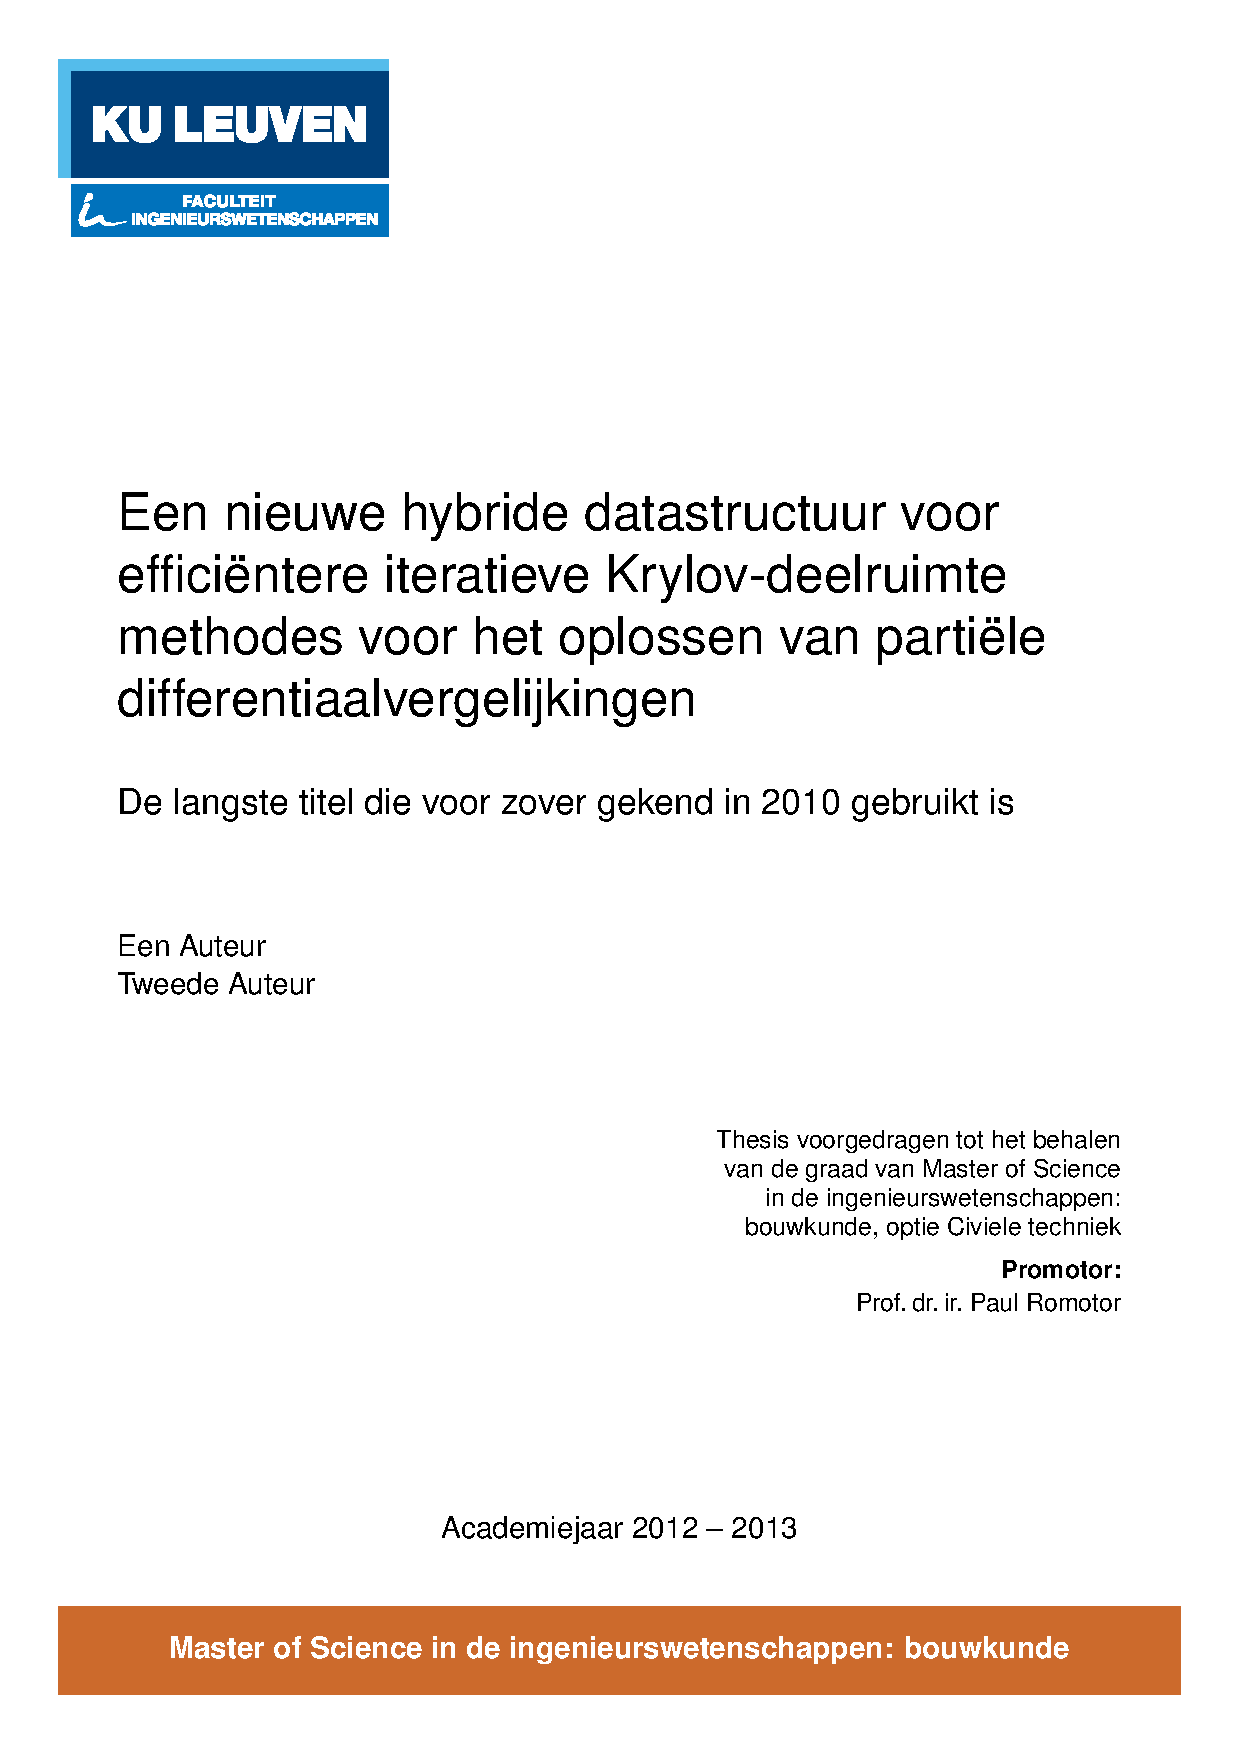
\includegraphics[width=\textwidth]{coverpage}}
  \caption{The official cover page layout}
  \label{fig:coverpage}
\end{figure}

The cover page uses color and it must be printed as such. The colors of the
banner containing the master degree are defined in \Sref{sec:mastercolors}.

\paragraph{Title page} The title page (\fref{fig:titlepage}) is the first
page of the actual document. It contains the same information as the cover
page as well as the complete jury names.
\begin{figure}
  \centering \fboxsep=0pt
  \fbox{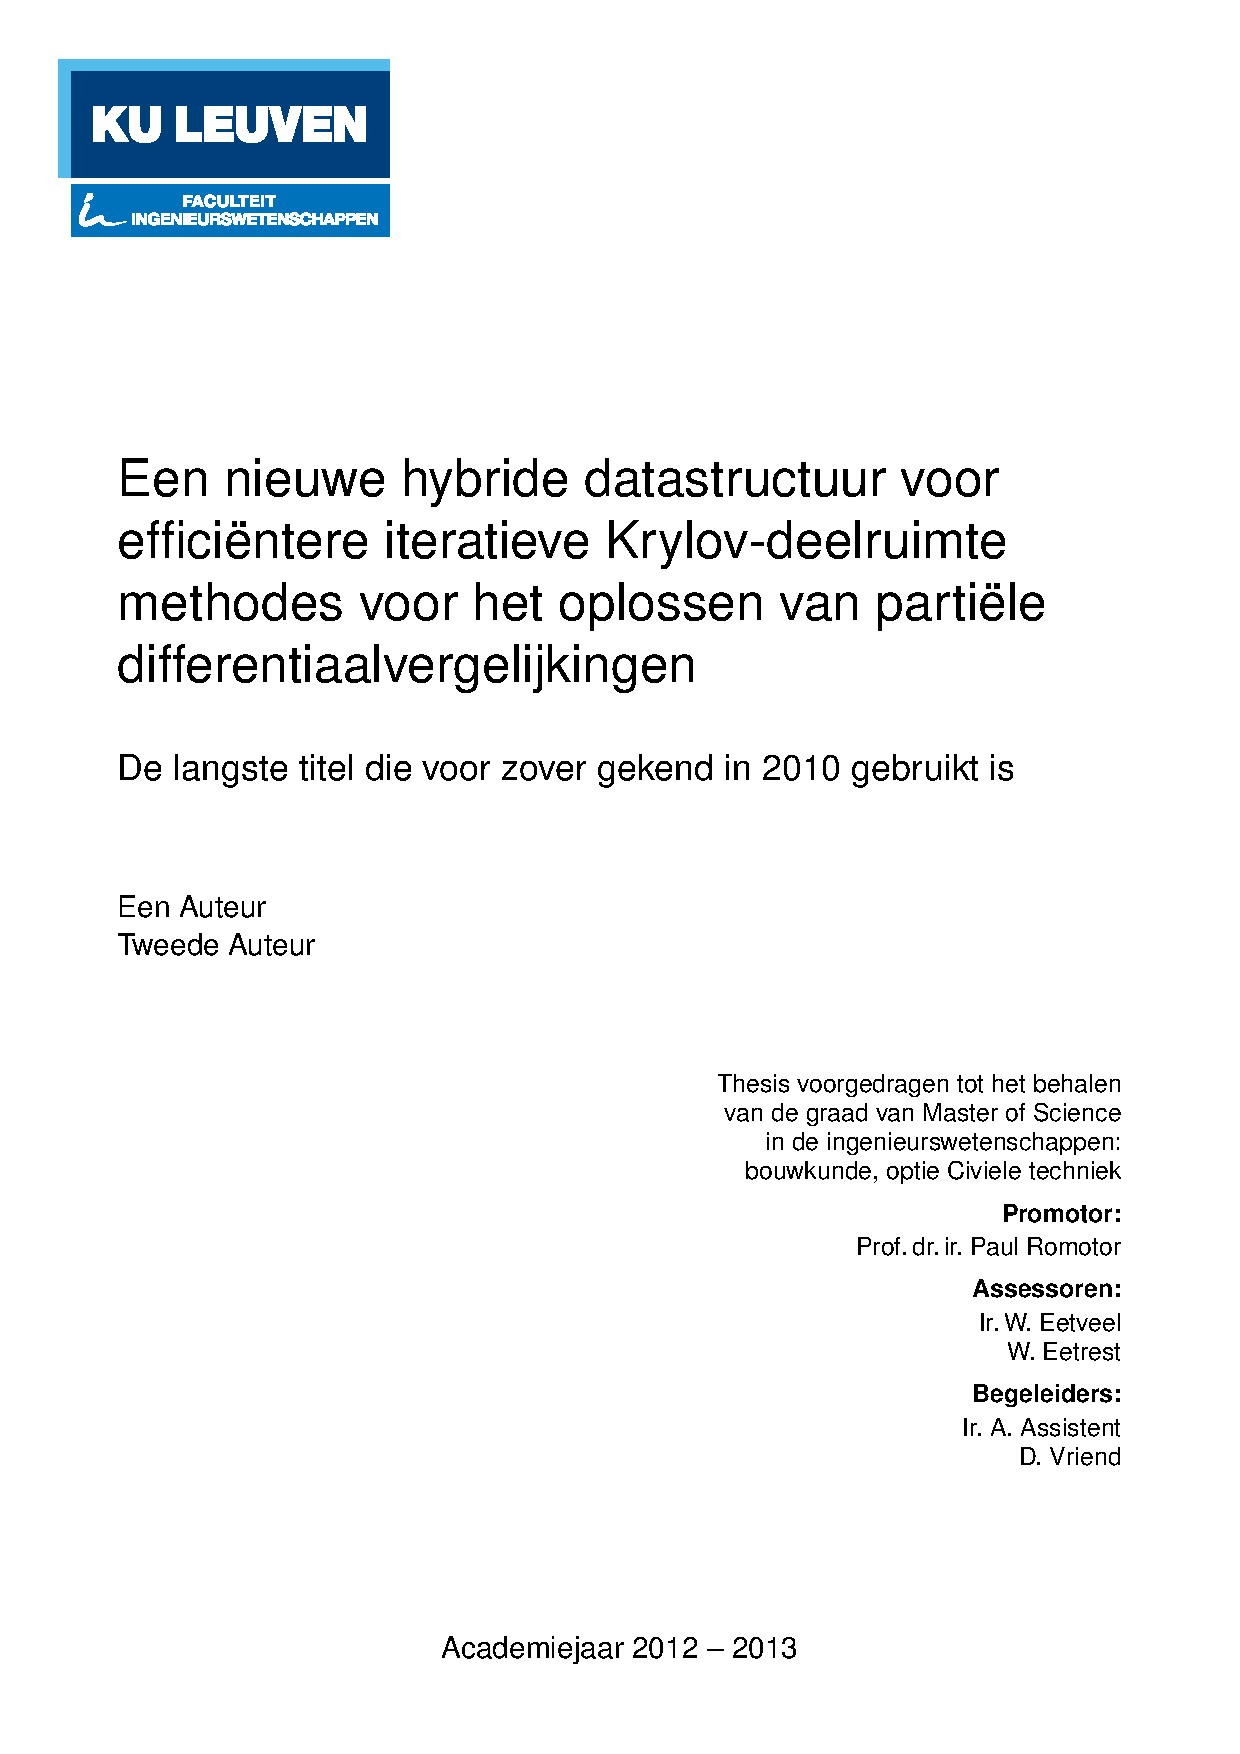
\includegraphics[width=\textwidth]{titlepage}}
  \caption{The official title page layout}
  \label{fig:titlepage}
\end{figure}

\paragraph{Copyright page} The copyright page (\fref{fig:copyright})
contains the necessary copyright statements and contact information. It is
printed on the verso side of the title page. If the text language differs
from the master language, an additional copyright statement in the text
language should be included.
\begin{figure}
  \centering \fboxsep=0pt
  \fbox{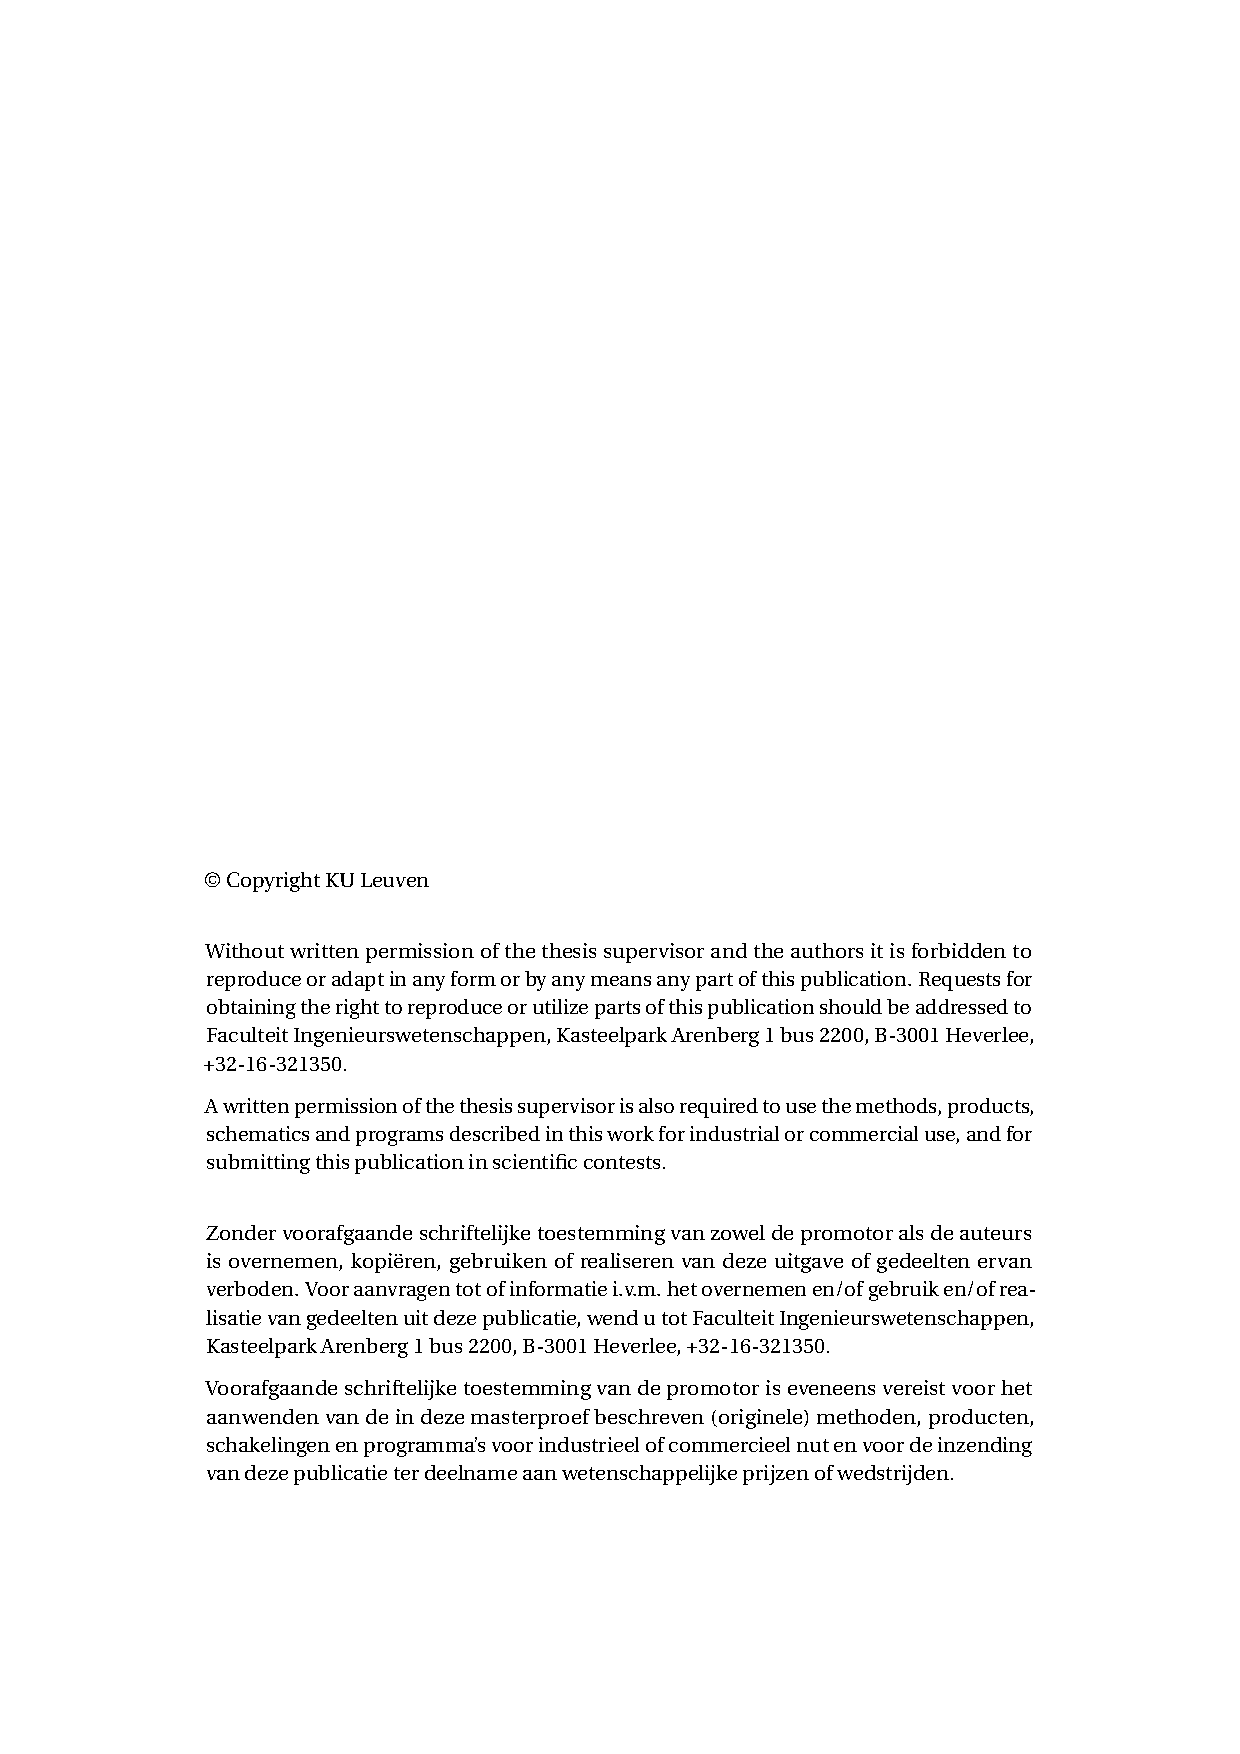
\includegraphics[width=\textwidth]{copyright}}
  \caption{The official copyright page layout}
  \label{fig:copyright}
\end{figure}

\section{Front matter}
The front matter contains introductory material such as a preface, an
abstract, and content lists (table of contents, list of tables, list of
figures, list of symbols, etc.).

\paragraph{Preface (\Dutch{Voorwoord})} The preface page contains personal
comments from the author(s). The preface can also be used for general
acknowledgments and to express one's thanks. This page is recommended but
not required.

\paragraph{Table of contents (\Dutch{Inhoudsopgave})} The table of contents
should be a clear representation of the breakdown of the chapters and the
respective page numbers. Don't show too many levels here since it will make
you loose the reader. So either restrict the table of contents to the
chapter and the section level or add the subsection level in an
unobstructive way.
% An example of the latter is the table of contents of this document, which
% tries to display the subsection level without attracting too much attention
% to it.

\paragraph{Abstract (\Dutch{Samenvatting})} The abstract page gives a one
page overview of the work emphasizing the results. Try to avoid uncommon
terminology, which will only be defined in the main text later on.

If the master language differs from the main text language, a second
abstract page is needed, which is written in the master language. This is
common practice for Erasmus students, where the main text language is
determined by the host institute. However if the master guidelines require
a multi-page abstract with figures, it's probably better to put it into an
appendix or into an additional chapter in the back matter.

\paragraph{List of figures (\Dutch{Lijst van figuren})} This list contains for each
figure its sequence number, its caption and its page number. Such a list is
often of limited use in a master thesis. Therefore it's not required
nor recommended unless the master guidelines require or recommend it.

\paragraph{List of tables (\Dutch{Lijst van tabellen})} This list contains for each
table its sequence number, its caption and its page number. The same remark
as for the list of figures is valid here.

\paragraph{Nomenclature (\Dutch{Lijst van symbolen})} This list holds the
nomenclature of the text. It shows all used symbols and abbreviations and
their meaning. Also conventions such as ``\emph{vectors are printed in
  bold}'' can be put in this list. This list is not required, but it is
recommended if some non-evident symbols or abbreviations are used. It's
useless to have a list of symbols indicating that $\alpha$ means the Greek
letter alpha!

\section{Main matter}
The main matter forms the heart of the thesis text: it contains the real
content. One should be able to read only the main matter to take in the
whole story. The main matter is divided into chapters, which are the
logical entities of the text. The chapters have a logical sequence, which
must be made evident to the reader.

\paragraph{First chapter} In this general introduction the reader must be
informed about the research field of the master thesis, situating it in a
broader context. The goals of the thesis, as well as previous work, are
described from a technical point of view. The structure of the thesis text
is briefly explained.

\paragraph{Other chapters} Each chapter, except the first and the last one,
starts with an introduction to the contents of the chapter. If a reader
would only read the introductions, he/she should have an overview of the
contents of the master thesis and the relation between the chapters.

Since chapters form a logical unit, it's expected that conclusions can be
drawn at the end of each chapter about the work described in it. A
concluding section can also help to link a chapter to the next one.

\paragraph{Last chapter} The general conclusion summarizes all results,
criticizes the methods used, and makes suggestions for further work. It
can't contain any new elements.

\paragraph{Appendices (\Dutch{Bijlagen})} The appendices clarify or
complete the text but are not an essential part of the work. Extra
information which is essential for future work is also included in
appendices. Typical examples are: program code and algorithms, detailed
schematics, equipment specifications, mathematical derivations and an
exhaustive argumentation.

If the master guidelines gives a page limit for the text, it usually only
includes the regular chapters, not the appendices. However appendices can't
be used to by-pass this page limit because the evaluation of the thesis is
mainly based on the regular chapters.

\section{Back matter}
The back matter conveys information ancillary to that in the main matter.
Typical examples are a bibliography and a glossary.

\paragraph{Bibliography} The bibliography lists all referenced material.
The format used for the bibliography items is probably determined by the
master guidelines or by the thesis supervisor. References are needed for all
statements that aren't proven in the thesis. However references to courses
are superfluous.

\paragraph{Filing card (\Dutch{Fiche})} Some masters, such as the ones
listed in \Sref{sec:fiche}, require a filing card (\fref{fig:fiche}) at the
end of the text.
\begin{figure}
  \centering \fboxsep=0pt
  \fbox{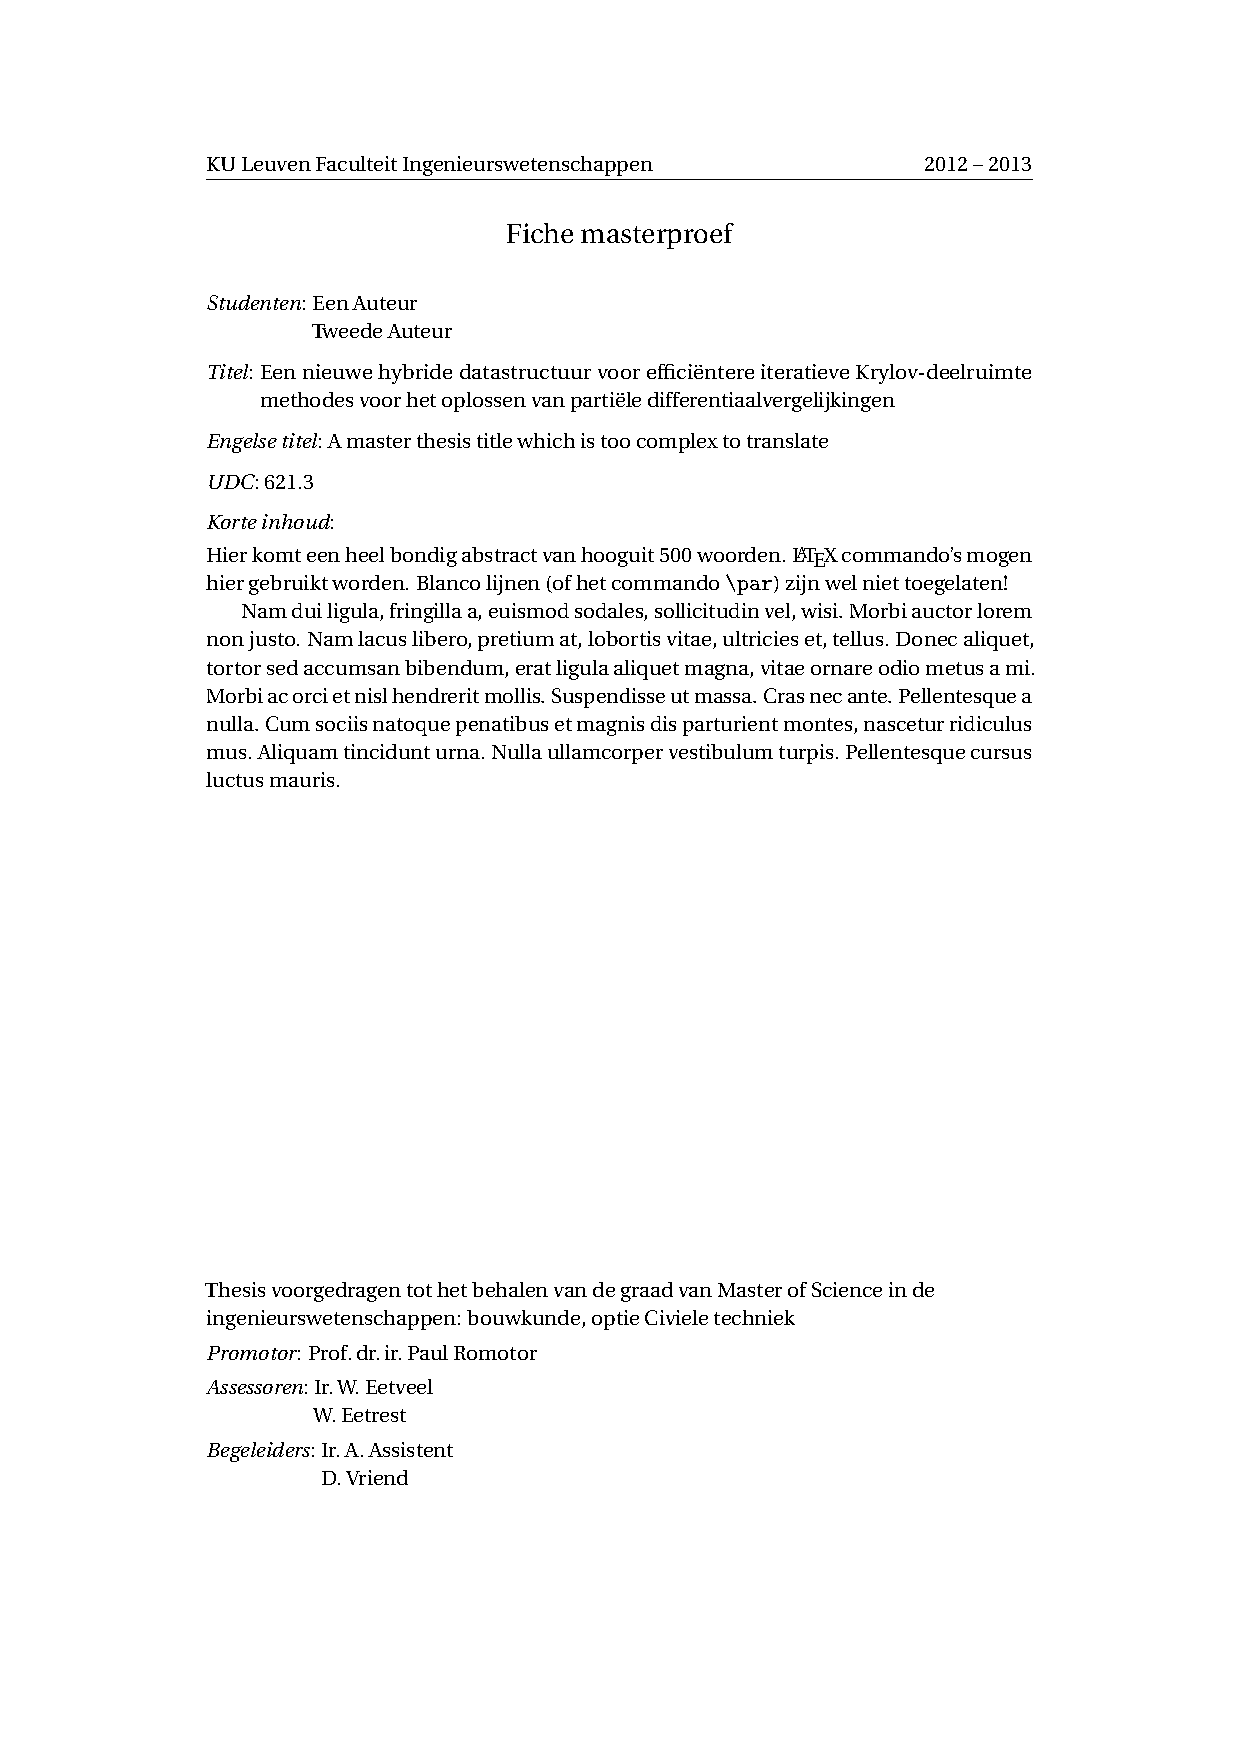
\includegraphics[width=\textwidth]{fiche}}
  \caption{The official filing card layout}
  \label{fig:fiche}
\end{figure}
It must contain all administrative information about the thesis: all
information from the title page, a translated title, UDC number, keywords,
title of the accompanying article, and a very short abstract (not longer
than 500 words). This page is typeset in the master language, with the
exception of the thesis title and the short abstract. It has a fixed
layout, just like the front pages. Therefore it must be generated in the
same way as the front pages: either with LaTeX or by getting a printed copy
from your master secretary.

\chapter{Typography}
A good first overall impression is always very important. Therefore
typography is a very important part of any masterpiece of text. And isn't
your master thesis a masterpiece?

Several good books have been written about typography and book design. A
(not so) short overview is found in the memoir design notes\,\cite{memdesign}.

\section{Basic principles}
The text must be written in a correct language, used in a consistent way.
Spelling mistakes are unacceptable, so at least use a decent spelling
checker. When in doubt, consult a dictionary or an official word list
(known in Dutch as the \Dutch{Groene Boekje}\,\cite{grboek}). A consistent
spelling implies that either British or American spelling is used when
writing an English text.

Consistency is also required for the grammar. Some sources suggest to use a
passive voice such as ``the results are found \ldots''. Other sources
suggest to rather use an active voice such as ``we found this result
\ldots''. Whatever you use, always try to stick to the same kind of
construction.

The master thesis should be written in a very readable way because it is
meant to communicate the results and scientific experience of the authors
to others.
Since a master thesis is a scientific work, official metric units (a.k.a.\
SI~units\,\cite{siunits}) must be used.
Identical concepts should be described with identical words or identical
symbols, as well in the body text and equations as in figures and tables.
To help the reader, it may be useful to add a list of symbols and
abbreviations in the front matter.

One sentence shouldn't contain more than one thought and is
therefore short. Ideas that belong together are kept together in one
paragraph. Therefore a paragraph usually contains at least two sentences,
spanning at least two lines.

\section{Fonts}
The body text is typeset using a proportional serif typeface. Well known
examples are Times\footnote{Since the typeface Times was developed for
  newspapers with small columns, it is not a good typeface for single
  column texts on A4 paper!} (or Times New Roman), Cambria, Palatino (or
Book Antiqua), Garamond, Utopia, Charter, and Minion. The font used in
formulas, figures, and tables must be the same as the body text font.
Symbols in the text and in formulas must be compatible with the chosen body
text font.

A general rule in typography is: \emph{``using fewer typefaces usually means
  better readability''}. But it makes sense to add one or two extra
typefaces for specific types of data to identify them more easily in
running text. To represent the name or contents of a file or a screen, one
typically uses a fixed width font, such as Courier or Consolas. For
non-body text (e.g., titles, headers, footers, captions) a proportional
sans serif font is sometimes used. Well known examples are Helvetica (or
Arial), Calibri, Univers, and Myriad. Just in case you're curious about it,
the fonts used in this document are \rmfontname, \texttt{\ttfontname}, and
\textsf{\sffontname}.

A font size of 11\,pt or 10\,pt with a proper leading\,\footnote{Leading is
  the vertical space between two lines of text. The line spacing is the
  font size plus the leading.} must be used for text and symbols. On A4
paper the 11\,pt size is preferred. If you don't know the proper leading
for your font, choose 2.5\,pt for the 11\,pt font and 2\,pt for the 10\,pt
font. Headings can be made more attractive and outstanding by typesetting
them in a larger font size and/or italics or bold.

\section{Layout}
The text is printed on both sides of A4 paper with odd numbered pages on
the recto\,\footnote{The recto page is the right-hand page of a printed
  book. The left-hand page is called the verso page.} side. This implies
that the inner margins (left on recto, right on verso) are smaller than the
outer margins. Contrary to printed books, electronic versions are often
only read from the screen, one page at a time. In the latter case it makes
more sense to have equal left and right margins.

A page contains a one column typeblock and optionally a header and a
footer. The typeblock contains the regular text, the tables and figures,
and the footnotes. To improve the readability of the text, the width of the
typeblock is limited to 14\,cm when using an 11\,pt font and to 13\,cm when
using a 10\,pt font.

The pages should be numbered consecutively, except for the front pages. It
is customary for front matter pages to use lowercase roman numbers and for
other pages to use arabic numbers. In this case the page number is reset
to~1 on the first page of the main matter.

Only chapters in the main matter are numbered: regular chapters with arabic
numbers and appendices with uppercase letters. Chapters in the front and
back matter are unnumbered.
Numbered chapters normally start on a recto page.
Inside a chapter, only sections and subsections are numbered, always with
arabic numbers. Too many document levels will confuse the reader instead of
helping him/her.

One should be able to unambiguously interpret the figures, tables and
equations and they should be numbered, preferably by chapter. Each
reference to equations, figures, and tables should mention the
corresponding number. Each figure should have a caption below it which
briefly indicates what is shown. The main text should refer at least once
to each figure and its content should be discussed in the text. The author
needs to do the interpretation of the figures, not the reader. The same is
true for tables, but traditionally the table caption is put above the table.

\chapter{Master specific data}
\begingroup
\makeatletter
\let\kulemt@end@master@def\endinput
\def\ProvidesFile#1[#2]{This section describes some master specific
  data as it was known on \printdateTeX{#2}.\par}
\let\kulemt@div@master\@gobble
\let\kulemt@def@master\@gobbletwo
\newcommand*\kulemt@obsolete@master[3][]{}
%% Configuration file for inclusion in kulemt.cls             -*- LaTeX -*-
%% This kulemt.cfg file holds all master dependent information for
%% the KU Leuven engineering master thesis class.
%% Author: Luc Van Eycken (Luc.VanEycken@esat.kuleuven.be)
%% If you modify this file:
%% * provide feedback to the original author
%% * please adjust the date [YYYY/MM/DD]
\ProvidesFile{kulemt.cfg}[2013/05/01]
%% Define known masters and their options
%%   The definition of the master contains the following elements:
%%    1. "N" or "E" : the language of the master
%%                    "N" for dutch, "E" for English
%%    2. Number for faculty identification (use braces if > 1 digit)
%%       0 = multiple faculties
%%       1 = Faculty of Engineering Science
%%    3. "F" or "N" : if "F", a filing card is always required
%%    4. Master colors "{bg:fg}" or "{bg}", with each color a comma
%%       separated list of C,M,Y,K fractions.
%%    5. Master title between braces
%%    6. Optional copyright contact info {<address>:<phone>:<email>}
%%       Use faculty information if empty
%%    7. Optional list of master option abbreviations
%%       Each option is surrounded by braces and consists of an
%%       abbreviation, followed by ":" and the title of the option.
%%       Optionally the list can start with a list of abbreviations
%%       between square brackets. If this list is not empty, an error
%%       is raised when no master option is specified by the student.
%%       If the list equals "-", no master options are allowed.
%%    8. Optional list of obsolete master option abbreviations.
%%       The list has the same format as the list of master options.
%%       You have to make sure that the abbreviations don't conflict
%%       with those of the master options. The convention is to append
%%       a dot and the last year it was valid.
%%
\kulemt@div@master{Dutch initial masters}
\kulemt@def@master{arc}{N1N{0.93,0.52,0.35,0.11:0,0,0,0}%
  {Master of Science in de ingenieurswetenschappen: architectuur}{}{[-]}}
\kulemt@def@master{bin}{N0N{}%
  {Master of Science in de bio-informatica}}
\kulemt@def@master{bmt}{N1N{0.6,0,0.3,0}%
  {Master of Science in de ingenieurswetenschappen:
   biomedische~technologie}}
\kulemt@def@master{bwk}{N1N{0.2,0.7,1,0:0,0,0,0}%
  {Master of Science in de ingenieurswetenschappen: bouwkunde}{}%
  {{ct:optie Civiele techniek}%
   {gt:optie Gebouwentechniek}%
   {vk:optie Verkeerskunde}}}
\kulemt@def@master{cit}{N1N{0.9,0.26,1,0.13:0,0,0,0}%
  {Master of Science in de ingenieurswetenschappen:
   chemische~technologie}{}%
  {{cbpe:optie Chemische en biochemische proces engineering}%
   {me:optie Milieu engineering}%
   {pe:optie Product engineering}}%
  {{cbr.2012:optie Chemische en biochemische reactorkunde}%
   {ct.2012:optie Chemische technologie}%
   {mv.2012:optie Milieu en veiligheid}}}
\kulemt@def@master{cws}{N1F{0,0,1,0}%
  {Master of Science in de ingenieurswetenschappen:
   computerwetenschappen}%
  {\kulemt@ifdutch{het}{the} Departement Computerwetenschappen,
   Celestijnenlaan 200A bus 2402, B-3001 Heverlee:%
   +32-16-327700:info@cs.kuleuven.be}%
  {{ai:hoofdspecialisatie Artifici\"ele intelligentie}%
   {ci:hoofdspecialisatie Computationele informatica}%
   {db:hoofdspecialisatie Databases}%
   {gs:hoofdspecialisatie Gedistribueerde systemen}%
   {mmc:hoofdspecialisatie Mens-machine communicatie}%
   {se:hoofdspecialisatie Software engineering}%
   {vs:hoofdspecialisatie Veilige software}}%
  {{ai.2011:optie Artifici\"ele intelligentie}%
   {gs.2011:optie Gedistribueerde systemen}%
   {mmc.2011:optie Mens-machine communicatie}%
   {vs.2011:optie Veilige software}}}
\kulemt@def@master{elt}{N1N{0,0.2,0.7,0}%
  {Master of Science in de ingenieurswetenschappen: elektrotechniek}%
  {ESAT, Kasteelpark Arenberg 10 postbus 2440,
   B-3001 Heverlee:+32-16-321130:info@esat.kuleuven.be}%
  {[eg,im]%
   {eg:optie Elektronica en ge\"{\i}ntegreerde schakelingen}%
   {im:optie Ingebedde systemen en multimedia}}%
  {{ge.2012:optie Ge\"{\i}ntegreerde elektronica}%
   {ms.2012:optie Multimedia en signaalverwerking}%
   {tt.2012:optie Telecommunicatie en telematica}}}
\kulemt@def@master{ene}{N1N{0.5,0,1,0}%
  {Master of Science in de ingenieurswetenschappen: energie}{}{[-]}}
\kulemt@obsolete@master{gmk}{N1N{0.8,0.6,0,0:0,0,0,0}%
  {Master of Science in de ingenieurswetenschappen:
   geotechniek en mijnbouwkunde}}
\kulemt@def@master{mtk}{N1N{0.3,0,0.3,0}%
  {Master of Science in de ingenieurswetenschappen: materiaalkunde}{}%
  {{mb:optie Materialen in de biomedische sector}%
   {mk:optie Metalen en keramieken}%
   {mn:optie Materialen voor nanotechnologie}%
   {pc:optie Polymeren en composieten}%
   {pp:optie Productie en processen}}}
\kulemt@def@master{vlit}{N1N{0,0,0.33,0}%
  {Master of Science in de ingenieurswetenschappen:
   verkeer, logistiek en intelligente transportsystemen}%
  {Centre for Industrial Management, Celestijnenlaan 300A Bus 2422,
   B-3001 Heverlee:+32-16-322567}%
  {{lt:optie Logistiek en transport}%
   {vi:optie Verkeer en Infrastructuur}}}
\kulemt@obsolete@master{mtw}{N0N{}%
  {Master in de milieutechnologie en de milieuwetenschappen}}
\kulemt@def@master{nan}{N1N{0,0.8,0.7,0:0,0,0,0}%
  {Master of Science in de nanowetenschappen en de nanotechnologie}{}%
  {{nm:optie Nanomaterialen en nanochemie}%
   {ne:optie Nano-elektronicaontwerp}%
   {nc:optie Nanocomponenten en nanofysica}%
   {nb:optie Nanobiotechnologie}}%
  {{bi.2014:afstudeerrichting bio-ingenieur}%
   {ir.2014:afstudeerrichting burgerlijk ingenieur}%
   {nw.2014:afstudeerrichting natuurwetenschappen}}}
\kulemt@def@master{sta}{N0N{}%
  {Master of Science in de Statistiek}{}%
  {{asm:specialisatie Algemene statistische methodologie}%
   {bm:specialisatie Biometrie}%
   {bs:specialisatie Business statistiek}%
   {is:specialisatie Industri\"ele statistiek}%
   {sgp:specialisatie Statistiek in de sociale, gedrags- en
        pedagogische wetenschappen}%
   {so:specialisatie Statistiek en onderwijs}}}
\kulemt@def@master{wit}{N1F{0.9,0.94,0.02,0.07:0,0,0,0}%
  {Master of Science in de ingenieurswetenschappen:
   wiskundige~ingenieurstechnieken}%
  {\kulemt@ifdutch{het}{the} Departement Computerwetenschappen,
   Celestijnenlaan 200A bus 2402, B-3001 Heverlee:%
   +32-16-327700:info@cs.kuleuven.be}}
\kulemt@def@master{wtk}{N1N{0.6,0.3,0,0:0,0,0,0}%
  {Master of Science in de ingenieurswetenschappen: werktuigkunde}{}{[-]}}
\kulemt@div@master{English initial masters}
\kulemt@def@master{ebmt}{E1N{0.6,0,0.3,0}%
  {Master of Science in Biomedical~Engineering}}
\kulemt@def@master{ebin}{E0N{}%
  {Master of Science in Bioinformatics}}
\kulemt@def@master{ecit}{E1N{0.9,0.26,1,0.13:0,0,0,0}%
  {Master of Science in Chemical~Engineering}{}%
  {{cbpe:option Chemical and biochemical process engineering}%
   {me:option Environmental engineering}%
   {pe:option Product engineering}}}
\kulemt@def@master{ect}{E1N{0.9,0.26,1,0.13:0,0,0,0}%
  {Master of Science in Chemical Engineering (Engineering Rheology)}}
\kulemt@def@master{ecws}{E1F{0,0,1,0}%
  {Master of Science in Engineering: Computer Science}%
  {\kulemt@ifdutch{het}{the} Departement Computerwetenschappen,
   Celestijnenlaan 200A bus 2402, B-3001 Heverlee:%
   +32-16-327700:info@cs.kuleuven.be}%
  {{ai:specialisation Artificial Intelligence}%
   {ss:specialisation Secure Software}}}
\kulemt@def@master{eelt}{E1N{0,0.2,0.7,0}%
  {Master of Science in Electrical~Engineering}%
  {Departement Elektrotechniek, Kasteelpark Arenberg 10 postbus 2440,
    B-3001 Heverlee:+32-16-321130:info@esat.kuleuven.be}%
  {[ei,em]%
   {ei:option Electronics and Integrated Circuits}%
   {em:option Embedded Systems and Multimedia}}}
\kulemt@def@master{eene}{E1N{0.5,0,1,0}%
  {Master of Science in Engineering: Energy}{}{[-]}}
\kulemt@def@master{ekene}{E1N{0.5,0,1,0}%
  {EIT-KIC Master in Energy}{}{[-]}}
\kulemt@def@master{ememn}{E1N{0.5,0,1,0}%
  {Erasmus Mundus Joint Master of Economics and
   Management of Network~Industries}}
\kulemt@def@master{emtk}{E1N{0.3,0,0.3,0}%
  {Master of Science in Materials Engineering}{}%
  {{mc:option Metals and Ceramics}%
   {mn:option Materials for Nanotechnology}%
   {pc:option Polymers and Composites}}}
\kulemt@def@master{enan}{E1N{0,0.8,0.7,0:0,0,0,0}%
  {Master of Science in Nanoscience and Nanotechnology}{}%
  {{nm:option Nanomaterials and Nanochemistry}%
   {ne:option Nanoelectronic Design}%
   {nd:option Nanodevices and Nanophysics}%
   {nb:option Nanobiotechnology}}%
  {{be.2014:major subject Bioscience engineering}%
   {eng.2014:major subject Engineering}%
   {ns.2014:major subject Natural sciences}}}
\kulemt@def@master{emnan}{E0N{0,0.8,0.7,0:0,0,0,0}%
  {Erasmus Mundus Master of Science in
   Nanoscience and Nanotechnology}{}%
  {{bb:graduation option Biophysics and Bionanotechnology}%
   {ne:graduation option Nanoelectronics}%
   {nn:graduation option Nanophysics and Nanochemistry}}}
\kulemt@def@master{esta}{E0N{}%
  {Master of Science in Statistics}{}%
  {{ars:option All Round Statistics}%
   {bm:option Biometrics}%
   {bs:option Business Statistics}%
   {gsm:option General Statistical Methodology}%
   {is:option Industrial Statistics}%
   {qas:abridged programme --
        Quantitative Analysis in the Social Sciences}%
   {sbe:option Social, Behavioral and Educational Statistics}}}
\kulemt@def@master{ewit}{E1F{0.9,0.94,0.02,0.07:0,0,0,0}%
  {Master of Science in Mathematical Engineering}%
  {\kulemt@ifdutch{het}{the} Departement Computerwetenschappen,
   Celestijnenlaan 200A bus 2402, B-3001 Heverlee:%
   +32-16-327700:info@cs.kuleuven.be}}
\kulemt@def@master{ewtk}{E1N{0.6,0.3,0,0:0,0,0,0}%
  {Master of Science in Mechanical Engineering}{}{[-]}}
\kulemt@div@master{Post-initial masters}
\kulemt@def@master{cms}{E1N{}%
  {Master of Science in Conservation of Monuments and Sites}}
\kulemt@def@master{mai}{E0N{}%
  {Master of Science in Artificial Intelligence}%
  {\kulemt@ifdutch{het}{the} Departement Computerwetenschappen,
   Celestijnenlaan 200A bus 2402, B-3001 Heverlee:%
   +32-16-327700:info@cs.kuleuven.be}%
  {{cs:option Cognitive Science}%
   {ecs:option Engineering and Computer Science}%
   {slt:option Speech and Language Technology}}}
\kulemt@def@master{mhs}{E1N{}%
  {Master of Science in Human Settlements}}
\kulemt@obsolete@master{mim}{E1N{}%
  {Master of Industrial Management}{}%
  {{ese:option Environment, Safety and Energy}%
   {ict:option Information and Communication Technology}%
   {plp:option Production and Logistics Planning}}}
\kulemt@def@master{mms}{N0N{}%
  {Master of Science in de medische stralingsfysica}}
\kulemt@def@master{mne}{E1N{}%
  {Master of Science in Nuclear Engineering}}
\kulemt@def@master{mse}{E1N{}%
  {Master of Science in Safety Engineering}{}
  {[p,ps]%
   {p:option Prevention}%
   {ps:option Process Safety}}}
\kulemt@def@master{mss}{E0N{}%
  {Master of Science in Space Studies}{}%
  {{slpbm:major subject: Space Law, Policy, Business and Management}%
   {ss:major subject: Space Sciences}%
   {sta:major Subject: Space Technology and Applications}}}
\kulemt@obsolete@master{mvt}{N1N{}%
  {Master in de veiligheidstechniek}}
\kulemt@def@master{usp}{E1N{}%
  {Master of Science in Urbanism and Strategic Planning}{}%
  {{sp:option Spatial Planning}%
   {u:option Urbanism}}}
\kulemt@end@master@def
\def\kulemt@paa@#1{%
  \ifcase #1%
    \kulemt@ifdutch
      {Promotor\kulemt@ifand\kulemt@promotor{en}{}}%
      {Thesis supervisor\kulemt@ifand\kulemt@promotor{s}{}}%
  \or
    \kulemt@ifdutch
      {Assessor\kulemt@ifand\kulemt@assessor{en}{}}%
      {Assessor\kulemt@ifand\kulemt@assessor{s}{}}%
  \or
    \kulemt@ifdutch
      {Begeleider\kulemt@ifand\kulemt@assistant{s}{}}%
      {Mentor\kulemt@ifand\kulemt@assistant{s}{}}%
  \fi}
\endinput
%%
%% End of file `kulemt.cfg'.

\endgroup

\section{Specifying the master option}
Most masters allow you to specify your master option (\Dutch{optie}) or
major topic (\Dutch{afstudeerrichting}) of the master degree, if you want.
But there are some exceptions:
\begin{itemize}
\item The following masters are known to \emph{oblige} you to mention the
  master option or major topic on the front pages:
  \begingroup
  \makeatletter
  \let\kulemt@end@master@def\endinput
  \let\kulemt@div@master\@gobble
  \newcommand*\kulemt@obsolete@master[3][]{}
  \newcommand*\kulemt@def@master[2]{\HandleItem#2{}{}\@nil}
  \def\kulemt@set@mo[#1]#2\@nil{\def\@tempa{#1}}
  \def\HandleItem#1#2#3#4#5#6#7#8\@nil{%
    \@ifnextchar[\kulemt@set@mo{\kulemt@set@mo[]}#7\@nil
    \ifx\@tempa\@empty\else
      \def\@tempb{-}\ifx\@tempa\@tempb\else \item #5\fi\fi}
  \begin{itemize}
    %% Configuration file for inclusion in kulemt.cls             -*- LaTeX -*-
%% This kulemt.cfg file holds all master dependent information for
%% the KU Leuven engineering master thesis class.
%% Author: Luc Van Eycken (Luc.VanEycken@esat.kuleuven.be)
%% If you modify this file:
%% * provide feedback to the original author
%% * please adjust the date [YYYY/MM/DD]
\ProvidesFile{kulemt.cfg}[2013/05/01]
%% Define known masters and their options
%%   The definition of the master contains the following elements:
%%    1. "N" or "E" : the language of the master
%%                    "N" for dutch, "E" for English
%%    2. Number for faculty identification (use braces if > 1 digit)
%%       0 = multiple faculties
%%       1 = Faculty of Engineering Science
%%    3. "F" or "N" : if "F", a filing card is always required
%%    4. Master colors "{bg:fg}" or "{bg}", with each color a comma
%%       separated list of C,M,Y,K fractions.
%%    5. Master title between braces
%%    6. Optional copyright contact info {<address>:<phone>:<email>}
%%       Use faculty information if empty
%%    7. Optional list of master option abbreviations
%%       Each option is surrounded by braces and consists of an
%%       abbreviation, followed by ":" and the title of the option.
%%       Optionally the list can start with a list of abbreviations
%%       between square brackets. If this list is not empty, an error
%%       is raised when no master option is specified by the student.
%%       If the list equals "-", no master options are allowed.
%%    8. Optional list of obsolete master option abbreviations.
%%       The list has the same format as the list of master options.
%%       You have to make sure that the abbreviations don't conflict
%%       with those of the master options. The convention is to append
%%       a dot and the last year it was valid.
%%
\kulemt@div@master{Dutch initial masters}
\kulemt@def@master{arc}{N1N{0.93,0.52,0.35,0.11:0,0,0,0}%
  {Master of Science in de ingenieurswetenschappen: architectuur}{}{[-]}}
\kulemt@def@master{bin}{N0N{}%
  {Master of Science in de bio-informatica}}
\kulemt@def@master{bmt}{N1N{0.6,0,0.3,0}%
  {Master of Science in de ingenieurswetenschappen:
   biomedische~technologie}}
\kulemt@def@master{bwk}{N1N{0.2,0.7,1,0:0,0,0,0}%
  {Master of Science in de ingenieurswetenschappen: bouwkunde}{}%
  {{ct:optie Civiele techniek}%
   {gt:optie Gebouwentechniek}%
   {vk:optie Verkeerskunde}}}
\kulemt@def@master{cit}{N1N{0.9,0.26,1,0.13:0,0,0,0}%
  {Master of Science in de ingenieurswetenschappen:
   chemische~technologie}{}%
  {{cbpe:optie Chemische en biochemische proces engineering}%
   {me:optie Milieu engineering}%
   {pe:optie Product engineering}}%
  {{cbr.2012:optie Chemische en biochemische reactorkunde}%
   {ct.2012:optie Chemische technologie}%
   {mv.2012:optie Milieu en veiligheid}}}
\kulemt@def@master{cws}{N1F{0,0,1,0}%
  {Master of Science in de ingenieurswetenschappen:
   computerwetenschappen}%
  {\kulemt@ifdutch{het}{the} Departement Computerwetenschappen,
   Celestijnenlaan 200A bus 2402, B-3001 Heverlee:%
   +32-16-327700:info@cs.kuleuven.be}%
  {{ai:hoofdspecialisatie Artifici\"ele intelligentie}%
   {ci:hoofdspecialisatie Computationele informatica}%
   {db:hoofdspecialisatie Databases}%
   {gs:hoofdspecialisatie Gedistribueerde systemen}%
   {mmc:hoofdspecialisatie Mens-machine communicatie}%
   {se:hoofdspecialisatie Software engineering}%
   {vs:hoofdspecialisatie Veilige software}}%
  {{ai.2011:optie Artifici\"ele intelligentie}%
   {gs.2011:optie Gedistribueerde systemen}%
   {mmc.2011:optie Mens-machine communicatie}%
   {vs.2011:optie Veilige software}}}
\kulemt@def@master{elt}{N1N{0,0.2,0.7,0}%
  {Master of Science in de ingenieurswetenschappen: elektrotechniek}%
  {ESAT, Kasteelpark Arenberg 10 postbus 2440,
   B-3001 Heverlee:+32-16-321130:info@esat.kuleuven.be}%
  {[eg,im]%
   {eg:optie Elektronica en ge\"{\i}ntegreerde schakelingen}%
   {im:optie Ingebedde systemen en multimedia}}%
  {{ge.2012:optie Ge\"{\i}ntegreerde elektronica}%
   {ms.2012:optie Multimedia en signaalverwerking}%
   {tt.2012:optie Telecommunicatie en telematica}}}
\kulemt@def@master{ene}{N1N{0.5,0,1,0}%
  {Master of Science in de ingenieurswetenschappen: energie}{}{[-]}}
\kulemt@obsolete@master{gmk}{N1N{0.8,0.6,0,0:0,0,0,0}%
  {Master of Science in de ingenieurswetenschappen:
   geotechniek en mijnbouwkunde}}
\kulemt@def@master{mtk}{N1N{0.3,0,0.3,0}%
  {Master of Science in de ingenieurswetenschappen: materiaalkunde}{}%
  {{mb:optie Materialen in de biomedische sector}%
   {mk:optie Metalen en keramieken}%
   {mn:optie Materialen voor nanotechnologie}%
   {pc:optie Polymeren en composieten}%
   {pp:optie Productie en processen}}}
\kulemt@def@master{vlit}{N1N{0,0,0.33,0}%
  {Master of Science in de ingenieurswetenschappen:
   verkeer, logistiek en intelligente transportsystemen}%
  {Centre for Industrial Management, Celestijnenlaan 300A Bus 2422,
   B-3001 Heverlee:+32-16-322567}%
  {{lt:optie Logistiek en transport}%
   {vi:optie Verkeer en Infrastructuur}}}
\kulemt@obsolete@master{mtw}{N0N{}%
  {Master in de milieutechnologie en de milieuwetenschappen}}
\kulemt@def@master{nan}{N1N{0,0.8,0.7,0:0,0,0,0}%
  {Master of Science in de nanowetenschappen en de nanotechnologie}{}%
  {{nm:optie Nanomaterialen en nanochemie}%
   {ne:optie Nano-elektronicaontwerp}%
   {nc:optie Nanocomponenten en nanofysica}%
   {nb:optie Nanobiotechnologie}}%
  {{bi.2014:afstudeerrichting bio-ingenieur}%
   {ir.2014:afstudeerrichting burgerlijk ingenieur}%
   {nw.2014:afstudeerrichting natuurwetenschappen}}}
\kulemt@def@master{sta}{N0N{}%
  {Master of Science in de Statistiek}{}%
  {{asm:specialisatie Algemene statistische methodologie}%
   {bm:specialisatie Biometrie}%
   {bs:specialisatie Business statistiek}%
   {is:specialisatie Industri\"ele statistiek}%
   {sgp:specialisatie Statistiek in de sociale, gedrags- en
        pedagogische wetenschappen}%
   {so:specialisatie Statistiek en onderwijs}}}
\kulemt@def@master{wit}{N1F{0.9,0.94,0.02,0.07:0,0,0,0}%
  {Master of Science in de ingenieurswetenschappen:
   wiskundige~ingenieurstechnieken}%
  {\kulemt@ifdutch{het}{the} Departement Computerwetenschappen,
   Celestijnenlaan 200A bus 2402, B-3001 Heverlee:%
   +32-16-327700:info@cs.kuleuven.be}}
\kulemt@def@master{wtk}{N1N{0.6,0.3,0,0:0,0,0,0}%
  {Master of Science in de ingenieurswetenschappen: werktuigkunde}{}{[-]}}
\kulemt@div@master{English initial masters}
\kulemt@def@master{ebmt}{E1N{0.6,0,0.3,0}%
  {Master of Science in Biomedical~Engineering}}
\kulemt@def@master{ebin}{E0N{}%
  {Master of Science in Bioinformatics}}
\kulemt@def@master{ecit}{E1N{0.9,0.26,1,0.13:0,0,0,0}%
  {Master of Science in Chemical~Engineering}{}%
  {{cbpe:option Chemical and biochemical process engineering}%
   {me:option Environmental engineering}%
   {pe:option Product engineering}}}
\kulemt@def@master{ect}{E1N{0.9,0.26,1,0.13:0,0,0,0}%
  {Master of Science in Chemical Engineering (Engineering Rheology)}}
\kulemt@def@master{ecws}{E1F{0,0,1,0}%
  {Master of Science in Engineering: Computer Science}%
  {\kulemt@ifdutch{het}{the} Departement Computerwetenschappen,
   Celestijnenlaan 200A bus 2402, B-3001 Heverlee:%
   +32-16-327700:info@cs.kuleuven.be}%
  {{ai:specialisation Artificial Intelligence}%
   {ss:specialisation Secure Software}}}
\kulemt@def@master{eelt}{E1N{0,0.2,0.7,0}%
  {Master of Science in Electrical~Engineering}%
  {Departement Elektrotechniek, Kasteelpark Arenberg 10 postbus 2440,
    B-3001 Heverlee:+32-16-321130:info@esat.kuleuven.be}%
  {[ei,em]%
   {ei:option Electronics and Integrated Circuits}%
   {em:option Embedded Systems and Multimedia}}}
\kulemt@def@master{eene}{E1N{0.5,0,1,0}%
  {Master of Science in Engineering: Energy}{}{[-]}}
\kulemt@def@master{ekene}{E1N{0.5,0,1,0}%
  {EIT-KIC Master in Energy}{}{[-]}}
\kulemt@def@master{ememn}{E1N{0.5,0,1,0}%
  {Erasmus Mundus Joint Master of Economics and
   Management of Network~Industries}}
\kulemt@def@master{emtk}{E1N{0.3,0,0.3,0}%
  {Master of Science in Materials Engineering}{}%
  {{mc:option Metals and Ceramics}%
   {mn:option Materials for Nanotechnology}%
   {pc:option Polymers and Composites}}}
\kulemt@def@master{enan}{E1N{0,0.8,0.7,0:0,0,0,0}%
  {Master of Science in Nanoscience and Nanotechnology}{}%
  {{nm:option Nanomaterials and Nanochemistry}%
   {ne:option Nanoelectronic Design}%
   {nd:option Nanodevices and Nanophysics}%
   {nb:option Nanobiotechnology}}%
  {{be.2014:major subject Bioscience engineering}%
   {eng.2014:major subject Engineering}%
   {ns.2014:major subject Natural sciences}}}
\kulemt@def@master{emnan}{E0N{0,0.8,0.7,0:0,0,0,0}%
  {Erasmus Mundus Master of Science in
   Nanoscience and Nanotechnology}{}%
  {{bb:graduation option Biophysics and Bionanotechnology}%
   {ne:graduation option Nanoelectronics}%
   {nn:graduation option Nanophysics and Nanochemistry}}}
\kulemt@def@master{esta}{E0N{}%
  {Master of Science in Statistics}{}%
  {{ars:option All Round Statistics}%
   {bm:option Biometrics}%
   {bs:option Business Statistics}%
   {gsm:option General Statistical Methodology}%
   {is:option Industrial Statistics}%
   {qas:abridged programme --
        Quantitative Analysis in the Social Sciences}%
   {sbe:option Social, Behavioral and Educational Statistics}}}
\kulemt@def@master{ewit}{E1F{0.9,0.94,0.02,0.07:0,0,0,0}%
  {Master of Science in Mathematical Engineering}%
  {\kulemt@ifdutch{het}{the} Departement Computerwetenschappen,
   Celestijnenlaan 200A bus 2402, B-3001 Heverlee:%
   +32-16-327700:info@cs.kuleuven.be}}
\kulemt@def@master{ewtk}{E1N{0.6,0.3,0,0:0,0,0,0}%
  {Master of Science in Mechanical Engineering}{}{[-]}}
\kulemt@div@master{Post-initial masters}
\kulemt@def@master{cms}{E1N{}%
  {Master of Science in Conservation of Monuments and Sites}}
\kulemt@def@master{mai}{E0N{}%
  {Master of Science in Artificial Intelligence}%
  {\kulemt@ifdutch{het}{the} Departement Computerwetenschappen,
   Celestijnenlaan 200A bus 2402, B-3001 Heverlee:%
   +32-16-327700:info@cs.kuleuven.be}%
  {{cs:option Cognitive Science}%
   {ecs:option Engineering and Computer Science}%
   {slt:option Speech and Language Technology}}}
\kulemt@def@master{mhs}{E1N{}%
  {Master of Science in Human Settlements}}
\kulemt@obsolete@master{mim}{E1N{}%
  {Master of Industrial Management}{}%
  {{ese:option Environment, Safety and Energy}%
   {ict:option Information and Communication Technology}%
   {plp:option Production and Logistics Planning}}}
\kulemt@def@master{mms}{N0N{}%
  {Master of Science in de medische stralingsfysica}}
\kulemt@def@master{mne}{E1N{}%
  {Master of Science in Nuclear Engineering}}
\kulemt@def@master{mse}{E1N{}%
  {Master of Science in Safety Engineering}{}
  {[p,ps]%
   {p:option Prevention}%
   {ps:option Process Safety}}}
\kulemt@def@master{mss}{E0N{}%
  {Master of Science in Space Studies}{}%
  {{slpbm:major subject: Space Law, Policy, Business and Management}%
   {ss:major subject: Space Sciences}%
   {sta:major Subject: Space Technology and Applications}}}
\kulemt@obsolete@master{mvt}{N1N{}%
  {Master in de veiligheidstechniek}}
\kulemt@def@master{usp}{E1N{}%
  {Master of Science in Urbanism and Strategic Planning}{}%
  {{sp:option Spatial Planning}%
   {u:option Urbanism}}}
\kulemt@end@master@def
\def\kulemt@paa@#1{%
  \ifcase #1%
    \kulemt@ifdutch
      {Promotor\kulemt@ifand\kulemt@promotor{en}{}}%
      {Thesis supervisor\kulemt@ifand\kulemt@promotor{s}{}}%
  \or
    \kulemt@ifdutch
      {Assessor\kulemt@ifand\kulemt@assessor{en}{}}%
      {Assessor\kulemt@ifand\kulemt@assessor{s}{}}%
  \or
    \kulemt@ifdutch
      {Begeleider\kulemt@ifand\kulemt@assistant{s}{}}%
      {Mentor\kulemt@ifand\kulemt@assistant{s}{}}%
  \fi}
\endinput
%%
%% End of file `kulemt.cfg'.

  \end{itemize}
  \endgroup
\item The following masters are known to \emph{disallow} you to mention the
  master option or major topic on the front pages:
  \begingroup
  \makeatletter
  \let\kulemt@end@master@def\endinput
  \let\kulemt@div@master\@gobble
  \newcommand*\kulemt@obsolete@master[3][]{}
  \newcommand*\kulemt@def@master[2]{\HandleItem#2{}{}\@nil}
  \def\kulemt@set@mo[#1]#2\@nil{\def\@tempa{#1}}
  \def\HandleItem#1#2#3#4#5#6#7#8\@nil{%
    \@ifnextchar[\kulemt@set@mo{\kulemt@set@mo[]}#7\@nil
    \def\@tempb{-}\ifx\@tempa\@tempb \item #5\fi}
  \begin{itemize}
    %% Configuration file for inclusion in kulemt.cls             -*- LaTeX -*-
%% This kulemt.cfg file holds all master dependent information for
%% the KU Leuven engineering master thesis class.
%% Author: Luc Van Eycken (Luc.VanEycken@esat.kuleuven.be)
%% If you modify this file:
%% * provide feedback to the original author
%% * please adjust the date [YYYY/MM/DD]
\ProvidesFile{kulemt.cfg}[2013/05/01]
%% Define known masters and their options
%%   The definition of the master contains the following elements:
%%    1. "N" or "E" : the language of the master
%%                    "N" for dutch, "E" for English
%%    2. Number for faculty identification (use braces if > 1 digit)
%%       0 = multiple faculties
%%       1 = Faculty of Engineering Science
%%    3. "F" or "N" : if "F", a filing card is always required
%%    4. Master colors "{bg:fg}" or "{bg}", with each color a comma
%%       separated list of C,M,Y,K fractions.
%%    5. Master title between braces
%%    6. Optional copyright contact info {<address>:<phone>:<email>}
%%       Use faculty information if empty
%%    7. Optional list of master option abbreviations
%%       Each option is surrounded by braces and consists of an
%%       abbreviation, followed by ":" and the title of the option.
%%       Optionally the list can start with a list of abbreviations
%%       between square brackets. If this list is not empty, an error
%%       is raised when no master option is specified by the student.
%%       If the list equals "-", no master options are allowed.
%%    8. Optional list of obsolete master option abbreviations.
%%       The list has the same format as the list of master options.
%%       You have to make sure that the abbreviations don't conflict
%%       with those of the master options. The convention is to append
%%       a dot and the last year it was valid.
%%
\kulemt@div@master{Dutch initial masters}
\kulemt@def@master{arc}{N1N{0.93,0.52,0.35,0.11:0,0,0,0}%
  {Master of Science in de ingenieurswetenschappen: architectuur}{}{[-]}}
\kulemt@def@master{bin}{N0N{}%
  {Master of Science in de bio-informatica}}
\kulemt@def@master{bmt}{N1N{0.6,0,0.3,0}%
  {Master of Science in de ingenieurswetenschappen:
   biomedische~technologie}}
\kulemt@def@master{bwk}{N1N{0.2,0.7,1,0:0,0,0,0}%
  {Master of Science in de ingenieurswetenschappen: bouwkunde}{}%
  {{ct:optie Civiele techniek}%
   {gt:optie Gebouwentechniek}%
   {vk:optie Verkeerskunde}}}
\kulemt@def@master{cit}{N1N{0.9,0.26,1,0.13:0,0,0,0}%
  {Master of Science in de ingenieurswetenschappen:
   chemische~technologie}{}%
  {{cbpe:optie Chemische en biochemische proces engineering}%
   {me:optie Milieu engineering}%
   {pe:optie Product engineering}}%
  {{cbr.2012:optie Chemische en biochemische reactorkunde}%
   {ct.2012:optie Chemische technologie}%
   {mv.2012:optie Milieu en veiligheid}}}
\kulemt@def@master{cws}{N1F{0,0,1,0}%
  {Master of Science in de ingenieurswetenschappen:
   computerwetenschappen}%
  {\kulemt@ifdutch{het}{the} Departement Computerwetenschappen,
   Celestijnenlaan 200A bus 2402, B-3001 Heverlee:%
   +32-16-327700:info@cs.kuleuven.be}%
  {{ai:hoofdspecialisatie Artifici\"ele intelligentie}%
   {ci:hoofdspecialisatie Computationele informatica}%
   {db:hoofdspecialisatie Databases}%
   {gs:hoofdspecialisatie Gedistribueerde systemen}%
   {mmc:hoofdspecialisatie Mens-machine communicatie}%
   {se:hoofdspecialisatie Software engineering}%
   {vs:hoofdspecialisatie Veilige software}}%
  {{ai.2011:optie Artifici\"ele intelligentie}%
   {gs.2011:optie Gedistribueerde systemen}%
   {mmc.2011:optie Mens-machine communicatie}%
   {vs.2011:optie Veilige software}}}
\kulemt@def@master{elt}{N1N{0,0.2,0.7,0}%
  {Master of Science in de ingenieurswetenschappen: elektrotechniek}%
  {ESAT, Kasteelpark Arenberg 10 postbus 2440,
   B-3001 Heverlee:+32-16-321130:info@esat.kuleuven.be}%
  {[eg,im]%
   {eg:optie Elektronica en ge\"{\i}ntegreerde schakelingen}%
   {im:optie Ingebedde systemen en multimedia}}%
  {{ge.2012:optie Ge\"{\i}ntegreerde elektronica}%
   {ms.2012:optie Multimedia en signaalverwerking}%
   {tt.2012:optie Telecommunicatie en telematica}}}
\kulemt@def@master{ene}{N1N{0.5,0,1,0}%
  {Master of Science in de ingenieurswetenschappen: energie}{}{[-]}}
\kulemt@obsolete@master{gmk}{N1N{0.8,0.6,0,0:0,0,0,0}%
  {Master of Science in de ingenieurswetenschappen:
   geotechniek en mijnbouwkunde}}
\kulemt@def@master{mtk}{N1N{0.3,0,0.3,0}%
  {Master of Science in de ingenieurswetenschappen: materiaalkunde}{}%
  {{mb:optie Materialen in de biomedische sector}%
   {mk:optie Metalen en keramieken}%
   {mn:optie Materialen voor nanotechnologie}%
   {pc:optie Polymeren en composieten}%
   {pp:optie Productie en processen}}}
\kulemt@def@master{vlit}{N1N{0,0,0.33,0}%
  {Master of Science in de ingenieurswetenschappen:
   verkeer, logistiek en intelligente transportsystemen}%
  {Centre for Industrial Management, Celestijnenlaan 300A Bus 2422,
   B-3001 Heverlee:+32-16-322567}%
  {{lt:optie Logistiek en transport}%
   {vi:optie Verkeer en Infrastructuur}}}
\kulemt@obsolete@master{mtw}{N0N{}%
  {Master in de milieutechnologie en de milieuwetenschappen}}
\kulemt@def@master{nan}{N1N{0,0.8,0.7,0:0,0,0,0}%
  {Master of Science in de nanowetenschappen en de nanotechnologie}{}%
  {{nm:optie Nanomaterialen en nanochemie}%
   {ne:optie Nano-elektronicaontwerp}%
   {nc:optie Nanocomponenten en nanofysica}%
   {nb:optie Nanobiotechnologie}}%
  {{bi.2014:afstudeerrichting bio-ingenieur}%
   {ir.2014:afstudeerrichting burgerlijk ingenieur}%
   {nw.2014:afstudeerrichting natuurwetenschappen}}}
\kulemt@def@master{sta}{N0N{}%
  {Master of Science in de Statistiek}{}%
  {{asm:specialisatie Algemene statistische methodologie}%
   {bm:specialisatie Biometrie}%
   {bs:specialisatie Business statistiek}%
   {is:specialisatie Industri\"ele statistiek}%
   {sgp:specialisatie Statistiek in de sociale, gedrags- en
        pedagogische wetenschappen}%
   {so:specialisatie Statistiek en onderwijs}}}
\kulemt@def@master{wit}{N1F{0.9,0.94,0.02,0.07:0,0,0,0}%
  {Master of Science in de ingenieurswetenschappen:
   wiskundige~ingenieurstechnieken}%
  {\kulemt@ifdutch{het}{the} Departement Computerwetenschappen,
   Celestijnenlaan 200A bus 2402, B-3001 Heverlee:%
   +32-16-327700:info@cs.kuleuven.be}}
\kulemt@def@master{wtk}{N1N{0.6,0.3,0,0:0,0,0,0}%
  {Master of Science in de ingenieurswetenschappen: werktuigkunde}{}{[-]}}
\kulemt@div@master{English initial masters}
\kulemt@def@master{ebmt}{E1N{0.6,0,0.3,0}%
  {Master of Science in Biomedical~Engineering}}
\kulemt@def@master{ebin}{E0N{}%
  {Master of Science in Bioinformatics}}
\kulemt@def@master{ecit}{E1N{0.9,0.26,1,0.13:0,0,0,0}%
  {Master of Science in Chemical~Engineering}{}%
  {{cbpe:option Chemical and biochemical process engineering}%
   {me:option Environmental engineering}%
   {pe:option Product engineering}}}
\kulemt@def@master{ect}{E1N{0.9,0.26,1,0.13:0,0,0,0}%
  {Master of Science in Chemical Engineering (Engineering Rheology)}}
\kulemt@def@master{ecws}{E1F{0,0,1,0}%
  {Master of Science in Engineering: Computer Science}%
  {\kulemt@ifdutch{het}{the} Departement Computerwetenschappen,
   Celestijnenlaan 200A bus 2402, B-3001 Heverlee:%
   +32-16-327700:info@cs.kuleuven.be}%
  {{ai:specialisation Artificial Intelligence}%
   {ss:specialisation Secure Software}}}
\kulemt@def@master{eelt}{E1N{0,0.2,0.7,0}%
  {Master of Science in Electrical~Engineering}%
  {Departement Elektrotechniek, Kasteelpark Arenberg 10 postbus 2440,
    B-3001 Heverlee:+32-16-321130:info@esat.kuleuven.be}%
  {[ei,em]%
   {ei:option Electronics and Integrated Circuits}%
   {em:option Embedded Systems and Multimedia}}}
\kulemt@def@master{eene}{E1N{0.5,0,1,0}%
  {Master of Science in Engineering: Energy}{}{[-]}}
\kulemt@def@master{ekene}{E1N{0.5,0,1,0}%
  {EIT-KIC Master in Energy}{}{[-]}}
\kulemt@def@master{ememn}{E1N{0.5,0,1,0}%
  {Erasmus Mundus Joint Master of Economics and
   Management of Network~Industries}}
\kulemt@def@master{emtk}{E1N{0.3,0,0.3,0}%
  {Master of Science in Materials Engineering}{}%
  {{mc:option Metals and Ceramics}%
   {mn:option Materials for Nanotechnology}%
   {pc:option Polymers and Composites}}}
\kulemt@def@master{enan}{E1N{0,0.8,0.7,0:0,0,0,0}%
  {Master of Science in Nanoscience and Nanotechnology}{}%
  {{nm:option Nanomaterials and Nanochemistry}%
   {ne:option Nanoelectronic Design}%
   {nd:option Nanodevices and Nanophysics}%
   {nb:option Nanobiotechnology}}%
  {{be.2014:major subject Bioscience engineering}%
   {eng.2014:major subject Engineering}%
   {ns.2014:major subject Natural sciences}}}
\kulemt@def@master{emnan}{E0N{0,0.8,0.7,0:0,0,0,0}%
  {Erasmus Mundus Master of Science in
   Nanoscience and Nanotechnology}{}%
  {{bb:graduation option Biophysics and Bionanotechnology}%
   {ne:graduation option Nanoelectronics}%
   {nn:graduation option Nanophysics and Nanochemistry}}}
\kulemt@def@master{esta}{E0N{}%
  {Master of Science in Statistics}{}%
  {{ars:option All Round Statistics}%
   {bm:option Biometrics}%
   {bs:option Business Statistics}%
   {gsm:option General Statistical Methodology}%
   {is:option Industrial Statistics}%
   {qas:abridged programme --
        Quantitative Analysis in the Social Sciences}%
   {sbe:option Social, Behavioral and Educational Statistics}}}
\kulemt@def@master{ewit}{E1F{0.9,0.94,0.02,0.07:0,0,0,0}%
  {Master of Science in Mathematical Engineering}%
  {\kulemt@ifdutch{het}{the} Departement Computerwetenschappen,
   Celestijnenlaan 200A bus 2402, B-3001 Heverlee:%
   +32-16-327700:info@cs.kuleuven.be}}
\kulemt@def@master{ewtk}{E1N{0.6,0.3,0,0:0,0,0,0}%
  {Master of Science in Mechanical Engineering}{}{[-]}}
\kulemt@div@master{Post-initial masters}
\kulemt@def@master{cms}{E1N{}%
  {Master of Science in Conservation of Monuments and Sites}}
\kulemt@def@master{mai}{E0N{}%
  {Master of Science in Artificial Intelligence}%
  {\kulemt@ifdutch{het}{the} Departement Computerwetenschappen,
   Celestijnenlaan 200A bus 2402, B-3001 Heverlee:%
   +32-16-327700:info@cs.kuleuven.be}%
  {{cs:option Cognitive Science}%
   {ecs:option Engineering and Computer Science}%
   {slt:option Speech and Language Technology}}}
\kulemt@def@master{mhs}{E1N{}%
  {Master of Science in Human Settlements}}
\kulemt@obsolete@master{mim}{E1N{}%
  {Master of Industrial Management}{}%
  {{ese:option Environment, Safety and Energy}%
   {ict:option Information and Communication Technology}%
   {plp:option Production and Logistics Planning}}}
\kulemt@def@master{mms}{N0N{}%
  {Master of Science in de medische stralingsfysica}}
\kulemt@def@master{mne}{E1N{}%
  {Master of Science in Nuclear Engineering}}
\kulemt@def@master{mse}{E1N{}%
  {Master of Science in Safety Engineering}{}
  {[p,ps]%
   {p:option Prevention}%
   {ps:option Process Safety}}}
\kulemt@def@master{mss}{E0N{}%
  {Master of Science in Space Studies}{}%
  {{slpbm:major subject: Space Law, Policy, Business and Management}%
   {ss:major subject: Space Sciences}%
   {sta:major Subject: Space Technology and Applications}}}
\kulemt@obsolete@master{mvt}{N1N{}%
  {Master in de veiligheidstechniek}}
\kulemt@def@master{usp}{E1N{}%
  {Master of Science in Urbanism and Strategic Planning}{}%
  {{sp:option Spatial Planning}%
   {u:option Urbanism}}}
\kulemt@end@master@def
\def\kulemt@paa@#1{%
  \ifcase #1%
    \kulemt@ifdutch
      {Promotor\kulemt@ifand\kulemt@promotor{en}{}}%
      {Thesis supervisor\kulemt@ifand\kulemt@promotor{s}{}}%
  \or
    \kulemt@ifdutch
      {Assessor\kulemt@ifand\kulemt@assessor{en}{}}%
      {Assessor\kulemt@ifand\kulemt@assessor{s}{}}%
  \or
    \kulemt@ifdutch
      {Begeleider\kulemt@ifand\kulemt@assistant{s}{}}%
      {Mentor\kulemt@ifand\kulemt@assistant{s}{}}%
  \fi}
\endinput
%%
%% End of file `kulemt.cfg'.

  \end{itemize}
  \endgroup
\end{itemize}

\section{Filing card}
\label{sec:fiche}
The following masters are known to require a filing card:
\begingroup
\makeatletter
\let\kulemt@end@master@def\endinput
\let\kulemt@div@master\@gobble
\newcommand*\kulemt@obsolete@master[3][]{}
\newcommand*\kulemt@def@master[2]{\HandleItem#2\@nil}
\def\HandleItem#1#2#3#4#5#6\@nil{%
  \if F\@car#3\@nil \item #5\fi}
\begin{itemize}
%% Configuration file for inclusion in kulemt.cls             -*- LaTeX -*-
%% This kulemt.cfg file holds all master dependent information for
%% the KU Leuven engineering master thesis class.
%% Author: Luc Van Eycken (Luc.VanEycken@esat.kuleuven.be)
%% If you modify this file:
%% * provide feedback to the original author
%% * please adjust the date [YYYY/MM/DD]
\ProvidesFile{kulemt.cfg}[2013/05/01]
%% Define known masters and their options
%%   The definition of the master contains the following elements:
%%    1. "N" or "E" : the language of the master
%%                    "N" for dutch, "E" for English
%%    2. Number for faculty identification (use braces if > 1 digit)
%%       0 = multiple faculties
%%       1 = Faculty of Engineering Science
%%    3. "F" or "N" : if "F", a filing card is always required
%%    4. Master colors "{bg:fg}" or "{bg}", with each color a comma
%%       separated list of C,M,Y,K fractions.
%%    5. Master title between braces
%%    6. Optional copyright contact info {<address>:<phone>:<email>}
%%       Use faculty information if empty
%%    7. Optional list of master option abbreviations
%%       Each option is surrounded by braces and consists of an
%%       abbreviation, followed by ":" and the title of the option.
%%       Optionally the list can start with a list of abbreviations
%%       between square brackets. If this list is not empty, an error
%%       is raised when no master option is specified by the student.
%%       If the list equals "-", no master options are allowed.
%%    8. Optional list of obsolete master option abbreviations.
%%       The list has the same format as the list of master options.
%%       You have to make sure that the abbreviations don't conflict
%%       with those of the master options. The convention is to append
%%       a dot and the last year it was valid.
%%
\kulemt@div@master{Dutch initial masters}
\kulemt@def@master{arc}{N1N{0.93,0.52,0.35,0.11:0,0,0,0}%
  {Master of Science in de ingenieurswetenschappen: architectuur}{}{[-]}}
\kulemt@def@master{bin}{N0N{}%
  {Master of Science in de bio-informatica}}
\kulemt@def@master{bmt}{N1N{0.6,0,0.3,0}%
  {Master of Science in de ingenieurswetenschappen:
   biomedische~technologie}}
\kulemt@def@master{bwk}{N1N{0.2,0.7,1,0:0,0,0,0}%
  {Master of Science in de ingenieurswetenschappen: bouwkunde}{}%
  {{ct:optie Civiele techniek}%
   {gt:optie Gebouwentechniek}%
   {vk:optie Verkeerskunde}}}
\kulemt@def@master{cit}{N1N{0.9,0.26,1,0.13:0,0,0,0}%
  {Master of Science in de ingenieurswetenschappen:
   chemische~technologie}{}%
  {{cbpe:optie Chemische en biochemische proces engineering}%
   {me:optie Milieu engineering}%
   {pe:optie Product engineering}}%
  {{cbr.2012:optie Chemische en biochemische reactorkunde}%
   {ct.2012:optie Chemische technologie}%
   {mv.2012:optie Milieu en veiligheid}}}
\kulemt@def@master{cws}{N1F{0,0,1,0}%
  {Master of Science in de ingenieurswetenschappen:
   computerwetenschappen}%
  {\kulemt@ifdutch{het}{the} Departement Computerwetenschappen,
   Celestijnenlaan 200A bus 2402, B-3001 Heverlee:%
   +32-16-327700:info@cs.kuleuven.be}%
  {{ai:hoofdspecialisatie Artifici\"ele intelligentie}%
   {ci:hoofdspecialisatie Computationele informatica}%
   {db:hoofdspecialisatie Databases}%
   {gs:hoofdspecialisatie Gedistribueerde systemen}%
   {mmc:hoofdspecialisatie Mens-machine communicatie}%
   {se:hoofdspecialisatie Software engineering}%
   {vs:hoofdspecialisatie Veilige software}}%
  {{ai.2011:optie Artifici\"ele intelligentie}%
   {gs.2011:optie Gedistribueerde systemen}%
   {mmc.2011:optie Mens-machine communicatie}%
   {vs.2011:optie Veilige software}}}
\kulemt@def@master{elt}{N1N{0,0.2,0.7,0}%
  {Master of Science in de ingenieurswetenschappen: elektrotechniek}%
  {ESAT, Kasteelpark Arenberg 10 postbus 2440,
   B-3001 Heverlee:+32-16-321130:info@esat.kuleuven.be}%
  {[eg,im]%
   {eg:optie Elektronica en ge\"{\i}ntegreerde schakelingen}%
   {im:optie Ingebedde systemen en multimedia}}%
  {{ge.2012:optie Ge\"{\i}ntegreerde elektronica}%
   {ms.2012:optie Multimedia en signaalverwerking}%
   {tt.2012:optie Telecommunicatie en telematica}}}
\kulemt@def@master{ene}{N1N{0.5,0,1,0}%
  {Master of Science in de ingenieurswetenschappen: energie}{}{[-]}}
\kulemt@obsolete@master{gmk}{N1N{0.8,0.6,0,0:0,0,0,0}%
  {Master of Science in de ingenieurswetenschappen:
   geotechniek en mijnbouwkunde}}
\kulemt@def@master{mtk}{N1N{0.3,0,0.3,0}%
  {Master of Science in de ingenieurswetenschappen: materiaalkunde}{}%
  {{mb:optie Materialen in de biomedische sector}%
   {mk:optie Metalen en keramieken}%
   {mn:optie Materialen voor nanotechnologie}%
   {pc:optie Polymeren en composieten}%
   {pp:optie Productie en processen}}}
\kulemt@def@master{vlit}{N1N{0,0,0.33,0}%
  {Master of Science in de ingenieurswetenschappen:
   verkeer, logistiek en intelligente transportsystemen}%
  {Centre for Industrial Management, Celestijnenlaan 300A Bus 2422,
   B-3001 Heverlee:+32-16-322567}%
  {{lt:optie Logistiek en transport}%
   {vi:optie Verkeer en Infrastructuur}}}
\kulemt@obsolete@master{mtw}{N0N{}%
  {Master in de milieutechnologie en de milieuwetenschappen}}
\kulemt@def@master{nan}{N1N{0,0.8,0.7,0:0,0,0,0}%
  {Master of Science in de nanowetenschappen en de nanotechnologie}{}%
  {{nm:optie Nanomaterialen en nanochemie}%
   {ne:optie Nano-elektronicaontwerp}%
   {nc:optie Nanocomponenten en nanofysica}%
   {nb:optie Nanobiotechnologie}}%
  {{bi.2014:afstudeerrichting bio-ingenieur}%
   {ir.2014:afstudeerrichting burgerlijk ingenieur}%
   {nw.2014:afstudeerrichting natuurwetenschappen}}}
\kulemt@def@master{sta}{N0N{}%
  {Master of Science in de Statistiek}{}%
  {{asm:specialisatie Algemene statistische methodologie}%
   {bm:specialisatie Biometrie}%
   {bs:specialisatie Business statistiek}%
   {is:specialisatie Industri\"ele statistiek}%
   {sgp:specialisatie Statistiek in de sociale, gedrags- en
        pedagogische wetenschappen}%
   {so:specialisatie Statistiek en onderwijs}}}
\kulemt@def@master{wit}{N1F{0.9,0.94,0.02,0.07:0,0,0,0}%
  {Master of Science in de ingenieurswetenschappen:
   wiskundige~ingenieurstechnieken}%
  {\kulemt@ifdutch{het}{the} Departement Computerwetenschappen,
   Celestijnenlaan 200A bus 2402, B-3001 Heverlee:%
   +32-16-327700:info@cs.kuleuven.be}}
\kulemt@def@master{wtk}{N1N{0.6,0.3,0,0:0,0,0,0}%
  {Master of Science in de ingenieurswetenschappen: werktuigkunde}{}{[-]}}
\kulemt@div@master{English initial masters}
\kulemt@def@master{ebmt}{E1N{0.6,0,0.3,0}%
  {Master of Science in Biomedical~Engineering}}
\kulemt@def@master{ebin}{E0N{}%
  {Master of Science in Bioinformatics}}
\kulemt@def@master{ecit}{E1N{0.9,0.26,1,0.13:0,0,0,0}%
  {Master of Science in Chemical~Engineering}{}%
  {{cbpe:option Chemical and biochemical process engineering}%
   {me:option Environmental engineering}%
   {pe:option Product engineering}}}
\kulemt@def@master{ect}{E1N{0.9,0.26,1,0.13:0,0,0,0}%
  {Master of Science in Chemical Engineering (Engineering Rheology)}}
\kulemt@def@master{ecws}{E1F{0,0,1,0}%
  {Master of Science in Engineering: Computer Science}%
  {\kulemt@ifdutch{het}{the} Departement Computerwetenschappen,
   Celestijnenlaan 200A bus 2402, B-3001 Heverlee:%
   +32-16-327700:info@cs.kuleuven.be}%
  {{ai:specialisation Artificial Intelligence}%
   {ss:specialisation Secure Software}}}
\kulemt@def@master{eelt}{E1N{0,0.2,0.7,0}%
  {Master of Science in Electrical~Engineering}%
  {Departement Elektrotechniek, Kasteelpark Arenberg 10 postbus 2440,
    B-3001 Heverlee:+32-16-321130:info@esat.kuleuven.be}%
  {[ei,em]%
   {ei:option Electronics and Integrated Circuits}%
   {em:option Embedded Systems and Multimedia}}}
\kulemt@def@master{eene}{E1N{0.5,0,1,0}%
  {Master of Science in Engineering: Energy}{}{[-]}}
\kulemt@def@master{ekene}{E1N{0.5,0,1,0}%
  {EIT-KIC Master in Energy}{}{[-]}}
\kulemt@def@master{ememn}{E1N{0.5,0,1,0}%
  {Erasmus Mundus Joint Master of Economics and
   Management of Network~Industries}}
\kulemt@def@master{emtk}{E1N{0.3,0,0.3,0}%
  {Master of Science in Materials Engineering}{}%
  {{mc:option Metals and Ceramics}%
   {mn:option Materials for Nanotechnology}%
   {pc:option Polymers and Composites}}}
\kulemt@def@master{enan}{E1N{0,0.8,0.7,0:0,0,0,0}%
  {Master of Science in Nanoscience and Nanotechnology}{}%
  {{nm:option Nanomaterials and Nanochemistry}%
   {ne:option Nanoelectronic Design}%
   {nd:option Nanodevices and Nanophysics}%
   {nb:option Nanobiotechnology}}%
  {{be.2014:major subject Bioscience engineering}%
   {eng.2014:major subject Engineering}%
   {ns.2014:major subject Natural sciences}}}
\kulemt@def@master{emnan}{E0N{0,0.8,0.7,0:0,0,0,0}%
  {Erasmus Mundus Master of Science in
   Nanoscience and Nanotechnology}{}%
  {{bb:graduation option Biophysics and Bionanotechnology}%
   {ne:graduation option Nanoelectronics}%
   {nn:graduation option Nanophysics and Nanochemistry}}}
\kulemt@def@master{esta}{E0N{}%
  {Master of Science in Statistics}{}%
  {{ars:option All Round Statistics}%
   {bm:option Biometrics}%
   {bs:option Business Statistics}%
   {gsm:option General Statistical Methodology}%
   {is:option Industrial Statistics}%
   {qas:abridged programme --
        Quantitative Analysis in the Social Sciences}%
   {sbe:option Social, Behavioral and Educational Statistics}}}
\kulemt@def@master{ewit}{E1F{0.9,0.94,0.02,0.07:0,0,0,0}%
  {Master of Science in Mathematical Engineering}%
  {\kulemt@ifdutch{het}{the} Departement Computerwetenschappen,
   Celestijnenlaan 200A bus 2402, B-3001 Heverlee:%
   +32-16-327700:info@cs.kuleuven.be}}
\kulemt@def@master{ewtk}{E1N{0.6,0.3,0,0:0,0,0,0}%
  {Master of Science in Mechanical Engineering}{}{[-]}}
\kulemt@div@master{Post-initial masters}
\kulemt@def@master{cms}{E1N{}%
  {Master of Science in Conservation of Monuments and Sites}}
\kulemt@def@master{mai}{E0N{}%
  {Master of Science in Artificial Intelligence}%
  {\kulemt@ifdutch{het}{the} Departement Computerwetenschappen,
   Celestijnenlaan 200A bus 2402, B-3001 Heverlee:%
   +32-16-327700:info@cs.kuleuven.be}%
  {{cs:option Cognitive Science}%
   {ecs:option Engineering and Computer Science}%
   {slt:option Speech and Language Technology}}}
\kulemt@def@master{mhs}{E1N{}%
  {Master of Science in Human Settlements}}
\kulemt@obsolete@master{mim}{E1N{}%
  {Master of Industrial Management}{}%
  {{ese:option Environment, Safety and Energy}%
   {ict:option Information and Communication Technology}%
   {plp:option Production and Logistics Planning}}}
\kulemt@def@master{mms}{N0N{}%
  {Master of Science in de medische stralingsfysica}}
\kulemt@def@master{mne}{E1N{}%
  {Master of Science in Nuclear Engineering}}
\kulemt@def@master{mse}{E1N{}%
  {Master of Science in Safety Engineering}{}
  {[p,ps]%
   {p:option Prevention}%
   {ps:option Process Safety}}}
\kulemt@def@master{mss}{E0N{}%
  {Master of Science in Space Studies}{}%
  {{slpbm:major subject: Space Law, Policy, Business and Management}%
   {ss:major subject: Space Sciences}%
   {sta:major Subject: Space Technology and Applications}}}
\kulemt@obsolete@master{mvt}{N1N{}%
  {Master in de veiligheidstechniek}}
\kulemt@def@master{usp}{E1N{}%
  {Master of Science in Urbanism and Strategic Planning}{}%
  {{sp:option Spatial Planning}%
   {u:option Urbanism}}}
\kulemt@end@master@def
\def\kulemt@paa@#1{%
  \ifcase #1%
    \kulemt@ifdutch
      {Promotor\kulemt@ifand\kulemt@promotor{en}{}}%
      {Thesis supervisor\kulemt@ifand\kulemt@promotor{s}{}}%
  \or
    \kulemt@ifdutch
      {Assessor\kulemt@ifand\kulemt@assessor{en}{}}%
      {Assessor\kulemt@ifand\kulemt@assessor{s}{}}%
  \or
    \kulemt@ifdutch
      {Begeleider\kulemt@ifand\kulemt@assistant{s}{}}%
      {Mentor\kulemt@ifand\kulemt@assistant{s}{}}%
  \fi}
\endinput
%%
%% End of file `kulemt.cfg'.

\end{itemize}
\endgroup

\section{Master colors}
\label{sec:mastercolors}
The master colors are shown below for all masters which have colors defined
by the Faculty of Engineering Science. These are the official colors, which
means that only the Faculty can change them. If a master wants to have its
colors added or changed, it should contact the Faculty secretary.

All colors are defined as coordinates in the \acro{CMYK} color space
which is normally used by printers. White corresponds to $(0,0,0,0)$ and
black to $(0,0,0,1)$ in \acro{CMYK}.

\begingroup
\makeatletter
\let\kulemt@end@master@def\endinput
\let\kulemt@div@master\@gobble
\newcommand*\kulemt@obsolete@master[3][]{}
\newcommand*\kulemt@def@master[2]{\HandleColors#2\@nil}
\def\HandleColors#1#2#3#4#5#6\@nil{%
  \if!#4!\else \par\bigskip
    \kulemt@getcolors #4::\@nil
    \centerline{\fboxsep\z@
      \expandafter\colorbox\kulemt@color@bg{%
        \vbox to 11mm{\vss \centering
          \fontfamily{phv}\fontseries\bfdefault\selectfont
          \expandafter\textcolor\kulemt@color@fg{#5}\vss}}}\nobreak
    \centerline{%
      Background color: \expandafter\printcolor\kulemt@color@bg\hfill
      Text color: \expandafter\printcolor\kulemt@color@fg}%
  \fi}
\def\kulemt@getcolors#1:#2:#3\@nil{%
  \edef\kulemt@color@bg{[cmyk]{\if !#1!0,0,0,0\else #1\fi}}%
  \edef\kulemt@color@fg{[cmyk]{\if !#2!0,0,0,1\else #2\fi}}}
\newcommand*\printcolor[2][]{$(#2)$}
%% Configuration file for inclusion in kulemt.cls             -*- LaTeX -*-
%% This kulemt.cfg file holds all master dependent information for
%% the KU Leuven engineering master thesis class.
%% Author: Luc Van Eycken (Luc.VanEycken@esat.kuleuven.be)
%% If you modify this file:
%% * provide feedback to the original author
%% * please adjust the date [YYYY/MM/DD]
\ProvidesFile{kulemt.cfg}[2013/05/01]
%% Define known masters and their options
%%   The definition of the master contains the following elements:
%%    1. "N" or "E" : the language of the master
%%                    "N" for dutch, "E" for English
%%    2. Number for faculty identification (use braces if > 1 digit)
%%       0 = multiple faculties
%%       1 = Faculty of Engineering Science
%%    3. "F" or "N" : if "F", a filing card is always required
%%    4. Master colors "{bg:fg}" or "{bg}", with each color a comma
%%       separated list of C,M,Y,K fractions.
%%    5. Master title between braces
%%    6. Optional copyright contact info {<address>:<phone>:<email>}
%%       Use faculty information if empty
%%    7. Optional list of master option abbreviations
%%       Each option is surrounded by braces and consists of an
%%       abbreviation, followed by ":" and the title of the option.
%%       Optionally the list can start with a list of abbreviations
%%       between square brackets. If this list is not empty, an error
%%       is raised when no master option is specified by the student.
%%       If the list equals "-", no master options are allowed.
%%    8. Optional list of obsolete master option abbreviations.
%%       The list has the same format as the list of master options.
%%       You have to make sure that the abbreviations don't conflict
%%       with those of the master options. The convention is to append
%%       a dot and the last year it was valid.
%%
\kulemt@div@master{Dutch initial masters}
\kulemt@def@master{arc}{N1N{0.93,0.52,0.35,0.11:0,0,0,0}%
  {Master of Science in de ingenieurswetenschappen: architectuur}{}{[-]}}
\kulemt@def@master{bin}{N0N{}%
  {Master of Science in de bio-informatica}}
\kulemt@def@master{bmt}{N1N{0.6,0,0.3,0}%
  {Master of Science in de ingenieurswetenschappen:
   biomedische~technologie}}
\kulemt@def@master{bwk}{N1N{0.2,0.7,1,0:0,0,0,0}%
  {Master of Science in de ingenieurswetenschappen: bouwkunde}{}%
  {{ct:optie Civiele techniek}%
   {gt:optie Gebouwentechniek}%
   {vk:optie Verkeerskunde}}}
\kulemt@def@master{cit}{N1N{0.9,0.26,1,0.13:0,0,0,0}%
  {Master of Science in de ingenieurswetenschappen:
   chemische~technologie}{}%
  {{cbpe:optie Chemische en biochemische proces engineering}%
   {me:optie Milieu engineering}%
   {pe:optie Product engineering}}%
  {{cbr.2012:optie Chemische en biochemische reactorkunde}%
   {ct.2012:optie Chemische technologie}%
   {mv.2012:optie Milieu en veiligheid}}}
\kulemt@def@master{cws}{N1F{0,0,1,0}%
  {Master of Science in de ingenieurswetenschappen:
   computerwetenschappen}%
  {\kulemt@ifdutch{het}{the} Departement Computerwetenschappen,
   Celestijnenlaan 200A bus 2402, B-3001 Heverlee:%
   +32-16-327700:info@cs.kuleuven.be}%
  {{ai:hoofdspecialisatie Artifici\"ele intelligentie}%
   {ci:hoofdspecialisatie Computationele informatica}%
   {db:hoofdspecialisatie Databases}%
   {gs:hoofdspecialisatie Gedistribueerde systemen}%
   {mmc:hoofdspecialisatie Mens-machine communicatie}%
   {se:hoofdspecialisatie Software engineering}%
   {vs:hoofdspecialisatie Veilige software}}%
  {{ai.2011:optie Artifici\"ele intelligentie}%
   {gs.2011:optie Gedistribueerde systemen}%
   {mmc.2011:optie Mens-machine communicatie}%
   {vs.2011:optie Veilige software}}}
\kulemt@def@master{elt}{N1N{0,0.2,0.7,0}%
  {Master of Science in de ingenieurswetenschappen: elektrotechniek}%
  {ESAT, Kasteelpark Arenberg 10 postbus 2440,
   B-3001 Heverlee:+32-16-321130:info@esat.kuleuven.be}%
  {[eg,im]%
   {eg:optie Elektronica en ge\"{\i}ntegreerde schakelingen}%
   {im:optie Ingebedde systemen en multimedia}}%
  {{ge.2012:optie Ge\"{\i}ntegreerde elektronica}%
   {ms.2012:optie Multimedia en signaalverwerking}%
   {tt.2012:optie Telecommunicatie en telematica}}}
\kulemt@def@master{ene}{N1N{0.5,0,1,0}%
  {Master of Science in de ingenieurswetenschappen: energie}{}{[-]}}
\kulemt@obsolete@master{gmk}{N1N{0.8,0.6,0,0:0,0,0,0}%
  {Master of Science in de ingenieurswetenschappen:
   geotechniek en mijnbouwkunde}}
\kulemt@def@master{mtk}{N1N{0.3,0,0.3,0}%
  {Master of Science in de ingenieurswetenschappen: materiaalkunde}{}%
  {{mb:optie Materialen in de biomedische sector}%
   {mk:optie Metalen en keramieken}%
   {mn:optie Materialen voor nanotechnologie}%
   {pc:optie Polymeren en composieten}%
   {pp:optie Productie en processen}}}
\kulemt@def@master{vlit}{N1N{0,0,0.33,0}%
  {Master of Science in de ingenieurswetenschappen:
   verkeer, logistiek en intelligente transportsystemen}%
  {Centre for Industrial Management, Celestijnenlaan 300A Bus 2422,
   B-3001 Heverlee:+32-16-322567}%
  {{lt:optie Logistiek en transport}%
   {vi:optie Verkeer en Infrastructuur}}}
\kulemt@obsolete@master{mtw}{N0N{}%
  {Master in de milieutechnologie en de milieuwetenschappen}}
\kulemt@def@master{nan}{N1N{0,0.8,0.7,0:0,0,0,0}%
  {Master of Science in de nanowetenschappen en de nanotechnologie}{}%
  {{nm:optie Nanomaterialen en nanochemie}%
   {ne:optie Nano-elektronicaontwerp}%
   {nc:optie Nanocomponenten en nanofysica}%
   {nb:optie Nanobiotechnologie}}%
  {{bi.2014:afstudeerrichting bio-ingenieur}%
   {ir.2014:afstudeerrichting burgerlijk ingenieur}%
   {nw.2014:afstudeerrichting natuurwetenschappen}}}
\kulemt@def@master{sta}{N0N{}%
  {Master of Science in de Statistiek}{}%
  {{asm:specialisatie Algemene statistische methodologie}%
   {bm:specialisatie Biometrie}%
   {bs:specialisatie Business statistiek}%
   {is:specialisatie Industri\"ele statistiek}%
   {sgp:specialisatie Statistiek in de sociale, gedrags- en
        pedagogische wetenschappen}%
   {so:specialisatie Statistiek en onderwijs}}}
\kulemt@def@master{wit}{N1F{0.9,0.94,0.02,0.07:0,0,0,0}%
  {Master of Science in de ingenieurswetenschappen:
   wiskundige~ingenieurstechnieken}%
  {\kulemt@ifdutch{het}{the} Departement Computerwetenschappen,
   Celestijnenlaan 200A bus 2402, B-3001 Heverlee:%
   +32-16-327700:info@cs.kuleuven.be}}
\kulemt@def@master{wtk}{N1N{0.6,0.3,0,0:0,0,0,0}%
  {Master of Science in de ingenieurswetenschappen: werktuigkunde}{}{[-]}}
\kulemt@div@master{English initial masters}
\kulemt@def@master{ebmt}{E1N{0.6,0,0.3,0}%
  {Master of Science in Biomedical~Engineering}}
\kulemt@def@master{ebin}{E0N{}%
  {Master of Science in Bioinformatics}}
\kulemt@def@master{ecit}{E1N{0.9,0.26,1,0.13:0,0,0,0}%
  {Master of Science in Chemical~Engineering}{}%
  {{cbpe:option Chemical and biochemical process engineering}%
   {me:option Environmental engineering}%
   {pe:option Product engineering}}}
\kulemt@def@master{ect}{E1N{0.9,0.26,1,0.13:0,0,0,0}%
  {Master of Science in Chemical Engineering (Engineering Rheology)}}
\kulemt@def@master{ecws}{E1F{0,0,1,0}%
  {Master of Science in Engineering: Computer Science}%
  {\kulemt@ifdutch{het}{the} Departement Computerwetenschappen,
   Celestijnenlaan 200A bus 2402, B-3001 Heverlee:%
   +32-16-327700:info@cs.kuleuven.be}%
  {{ai:specialisation Artificial Intelligence}%
   {ss:specialisation Secure Software}}}
\kulemt@def@master{eelt}{E1N{0,0.2,0.7,0}%
  {Master of Science in Electrical~Engineering}%
  {Departement Elektrotechniek, Kasteelpark Arenberg 10 postbus 2440,
    B-3001 Heverlee:+32-16-321130:info@esat.kuleuven.be}%
  {[ei,em]%
   {ei:option Electronics and Integrated Circuits}%
   {em:option Embedded Systems and Multimedia}}}
\kulemt@def@master{eene}{E1N{0.5,0,1,0}%
  {Master of Science in Engineering: Energy}{}{[-]}}
\kulemt@def@master{ekene}{E1N{0.5,0,1,0}%
  {EIT-KIC Master in Energy}{}{[-]}}
\kulemt@def@master{ememn}{E1N{0.5,0,1,0}%
  {Erasmus Mundus Joint Master of Economics and
   Management of Network~Industries}}
\kulemt@def@master{emtk}{E1N{0.3,0,0.3,0}%
  {Master of Science in Materials Engineering}{}%
  {{mc:option Metals and Ceramics}%
   {mn:option Materials for Nanotechnology}%
   {pc:option Polymers and Composites}}}
\kulemt@def@master{enan}{E1N{0,0.8,0.7,0:0,0,0,0}%
  {Master of Science in Nanoscience and Nanotechnology}{}%
  {{nm:option Nanomaterials and Nanochemistry}%
   {ne:option Nanoelectronic Design}%
   {nd:option Nanodevices and Nanophysics}%
   {nb:option Nanobiotechnology}}%
  {{be.2014:major subject Bioscience engineering}%
   {eng.2014:major subject Engineering}%
   {ns.2014:major subject Natural sciences}}}
\kulemt@def@master{emnan}{E0N{0,0.8,0.7,0:0,0,0,0}%
  {Erasmus Mundus Master of Science in
   Nanoscience and Nanotechnology}{}%
  {{bb:graduation option Biophysics and Bionanotechnology}%
   {ne:graduation option Nanoelectronics}%
   {nn:graduation option Nanophysics and Nanochemistry}}}
\kulemt@def@master{esta}{E0N{}%
  {Master of Science in Statistics}{}%
  {{ars:option All Round Statistics}%
   {bm:option Biometrics}%
   {bs:option Business Statistics}%
   {gsm:option General Statistical Methodology}%
   {is:option Industrial Statistics}%
   {qas:abridged programme --
        Quantitative Analysis in the Social Sciences}%
   {sbe:option Social, Behavioral and Educational Statistics}}}
\kulemt@def@master{ewit}{E1F{0.9,0.94,0.02,0.07:0,0,0,0}%
  {Master of Science in Mathematical Engineering}%
  {\kulemt@ifdutch{het}{the} Departement Computerwetenschappen,
   Celestijnenlaan 200A bus 2402, B-3001 Heverlee:%
   +32-16-327700:info@cs.kuleuven.be}}
\kulemt@def@master{ewtk}{E1N{0.6,0.3,0,0:0,0,0,0}%
  {Master of Science in Mechanical Engineering}{}{[-]}}
\kulemt@div@master{Post-initial masters}
\kulemt@def@master{cms}{E1N{}%
  {Master of Science in Conservation of Monuments and Sites}}
\kulemt@def@master{mai}{E0N{}%
  {Master of Science in Artificial Intelligence}%
  {\kulemt@ifdutch{het}{the} Departement Computerwetenschappen,
   Celestijnenlaan 200A bus 2402, B-3001 Heverlee:%
   +32-16-327700:info@cs.kuleuven.be}%
  {{cs:option Cognitive Science}%
   {ecs:option Engineering and Computer Science}%
   {slt:option Speech and Language Technology}}}
\kulemt@def@master{mhs}{E1N{}%
  {Master of Science in Human Settlements}}
\kulemt@obsolete@master{mim}{E1N{}%
  {Master of Industrial Management}{}%
  {{ese:option Environment, Safety and Energy}%
   {ict:option Information and Communication Technology}%
   {plp:option Production and Logistics Planning}}}
\kulemt@def@master{mms}{N0N{}%
  {Master of Science in de medische stralingsfysica}}
\kulemt@def@master{mne}{E1N{}%
  {Master of Science in Nuclear Engineering}}
\kulemt@def@master{mse}{E1N{}%
  {Master of Science in Safety Engineering}{}
  {[p,ps]%
   {p:option Prevention}%
   {ps:option Process Safety}}}
\kulemt@def@master{mss}{E0N{}%
  {Master of Science in Space Studies}{}%
  {{slpbm:major subject: Space Law, Policy, Business and Management}%
   {ss:major subject: Space Sciences}%
   {sta:major Subject: Space Technology and Applications}}}
\kulemt@obsolete@master{mvt}{N1N{}%
  {Master in de veiligheidstechniek}}
\kulemt@def@master{usp}{E1N{}%
  {Master of Science in Urbanism and Strategic Planning}{}%
  {{sp:option Spatial Planning}%
   {u:option Urbanism}}}
\kulemt@end@master@def
\def\kulemt@paa@#1{%
  \ifcase #1%
    \kulemt@ifdutch
      {Promotor\kulemt@ifand\kulemt@promotor{en}{}}%
      {Thesis supervisor\kulemt@ifand\kulemt@promotor{s}{}}%
  \or
    \kulemt@ifdutch
      {Assessor\kulemt@ifand\kulemt@assessor{en}{}}%
      {Assessor\kulemt@ifand\kulemt@assessor{s}{}}%
  \or
    \kulemt@ifdutch
      {Begeleider\kulemt@ifand\kulemt@assistant{s}{}}%
      {Mentor\kulemt@ifand\kulemt@assistant{s}{}}%
  \fi}
\endinput
%%
%% End of file `kulemt.cfg'.

\endgroup

\bibliographystyle{abbrvurl}
\bibliography{../manual/references}

\end{document}
